\documentclass[11pt]{article}

\usepackage[T1]{fontenc}
\usepackage[utf8]{inputenc}
\usepackage[margin=0.92in,headheight=15pt]{geometry}
\usepackage{amsmath,amsthm,mathtools}
\usepackage{newtxtext,newtxmath}
\usepackage{booktabs,array,tabularx}
\usepackage{enumitem}
\usepackage{microtype}
\usepackage{xcolor}
\usepackage{graphicx}
\usepackage{tikz}
\usepackage{tikz-cd}
\usetikzlibrary{arrows.meta,positioning,calc,fit,shapes.geometric,
  decorations.pathreplacing,backgrounds}
\usepackage[most]{tcolorbox}
\usepackage{fancyhdr}
\usepackage{titlesec}
\usepackage{caption}
\usepackage{etoolbox}
\usepackage[pagebackref]{hyperref}

\renewcommand{\contentsname}{\'Indice}
\renewcommand{\listfigurename}{\'Indice de figuras}
\renewcommand{\figurename}{Figura}
\renewcommand{\tablename}{Tabla}
\renewcommand{\proofname}{Demostraci\'on}
\renewcommand{\refname}{Referencias}

\renewcommand*{\backref}[1]{}
\renewcommand*{\backrefsep}{, }
\renewcommand*{\backreftwosep}{ y }
\renewcommand*{\backreflastsep}{ y }
\renewcommand*{\backrefalt}[4]{%
  \ifcase #1\relax
  \or\hspace{0.25em}\textcolor{paperink!60}{\scriptsize Citada en la p\'agina #2.}%
  \else\hspace{0.25em}\textcolor{paperink!60}{\scriptsize Citada en las p\'aginas #2.}%
  \fi}

\definecolor{paperink}{HTML}{182230}
\definecolor{deepblue}{HTML}{173B57}
\definecolor{teal}{HTML}{177E89}
\definecolor{gold}{HTML}{C7922E}
\definecolor{softblue}{HTML}{EEF5F8}
\definecolor{softgold}{HTML}{FBF5E8}
\definecolor{softgray}{HTML}{F4F6F7}

\newcommand{\paperdoi}{10.5281/zenodo.21460623}

\hypersetup{
  colorlinks=true,
  linkcolor=deepblue,
  citecolor=teal!75!black,
  urlcolor=teal!75!black,
  pdftitle={Ahora sabemos que siempre era demasiado optimista},
  pdfauthor={Javier Aragon},
  pdfsubject={Geometria algebraica y aplicaciones de Keller},
  pdfkeywords={Jacobian conjecture, Keller maps, nonproperness, cubic fibers},
  pdfinfo={DOI={10.5281/zenodo.21460623},
    DOIStatus={Reserved DOI -- pending publication}}
}

\color{paperink}
\setlength{\parindent}{0pt}
\setlength{\parskip}{0.48\baselineskip}
\setlist{itemsep=0.22em,topsep=0.35em,leftmargin=1.55em}
\setcounter{tocdepth}{2}

\titleformat{\part}[display]
  {\centering\sffamily\bfseries\color{deepblue}}
  {\Large PARTE \thepart}{0.5em}{\Huge}
\titlespacing*{\part}{0pt}{1.5em}{2.5em}
\titleformat{\section}
  {\Large\sffamily\bfseries\color{deepblue}}
  {\thesection}{0.75em}{}
\titleformat{\subsection}
  {\large\sffamily\bfseries\color{teal!75!black}}
  {\thesubsection}{0.65em}{}
\titleformat{\subsubsection}
  {\normalsize\sffamily\bfseries\color{paperink}}
  {\thesubsubsection}{0.6em}{}

\captionsetup{font=small,labelfont={bf,color=deepblue},
  textfont={color=paperink},justification=centering,skip=7pt}

\pagestyle{fancy}
\fancyhf{}
\fancyhead[L]{\small\sffamily\color{deepblue}Ahora sabemos que ``siempre'' era demasiado optimista}
\fancyhead[R]{\small\sffamily\color{teal!75!black}Javier Arag\'on}
\fancyfoot[C]{\small\sffamily\color{paperink!70}\thepage}
\renewcommand{\headrulewidth}{0.4pt}

\newtcolorbox{resultbox}[1]{enhanced,breakable,colback=softblue,
  colframe=deepblue,boxrule=0.8pt,arc=1.5mm,left=4mm,right=4mm,
  top=2.5mm,bottom=2.5mm,title={#1},fonttitle=\sffamily\bfseries,
  coltitle=white,colbacktitle=deepblue}
\newtcolorbox{insightbox}[1]{enhanced,breakable,colback=softgold,
  colframe=gold,boxrule=0.7pt,arc=1.5mm,left=4mm,right=4mm,
  top=2.5mm,bottom=2.5mm,title={#1},fonttitle=\sffamily\bfseries,
  coltitle=paperink,colbacktitle=gold!28}

\newtheorem{theorem}{Teorema}[section]
\newtheorem{proposition}[theorem]{Proposici\'on}
\newtheorem{lemma}[theorem]{Lema}
\newtheorem{corollary}[theorem]{Corolario}
\theoremstyle{definition}
\newtheorem{definition}[theorem]{Definici\'on}
\newtheorem{question}[theorem]{Pregunta}
\theoremstyle{remark}
\newtheorem{remark}[theorem]{Observaci\'on}

\newcommand{\C}{\mathbb{C}}
\newcommand{\Q}{\mathbb{Q}}
\newcommand{\A}{\mathbb{A}}
\newcommand{\Jac}{\operatorname{Jac}}
\newcommand{\Aut}{\operatorname{Aut}}
\newcommand{\Gal}{\operatorname{Gal}}
\newcommand{\Sing}{\operatorname{Sing}}
\newcommand{\bibauthor}[1]{\textsc{#1}}
\newcommand{\biblink}[2]{\href{#1}{\sffamily\footnotesize\color{teal!75!black}#2}}

\makeatletter
\renewcommand{\@biblabel}[1]{\textcolor{gold}{\sffamily\bfseries[#1]}}
\makeatother

\AtBeginEnvironment{thebibliography}{%
  \addcontentsline{toc}{section}{\refname}%
  \small
  \setlength{\itemsep}{0.7em}%
  \setlength{\parskip}{0.12em}%
}

\begin{document}
\pagenumbering{gobble}

\begin{titlepage}
\thispagestyle{empty}
\begin{tikzpicture}[remember picture,overlay]
  \fill[deepblue] (current page.north west) rectangle
    ([yshift=-1.15cm]current page.north east);
  \fill[teal!13] ([xshift=0.66\paperwidth]current page.south west)
    rectangle (current page.north east);
  \draw[deepblue!15,line width=1.2pt]
    ([xshift=-1.1cm,yshift=-1.5cm]current page.north east)
    .. controls +(-2.5,-1.2) and +(1.5,1.4) ..
    ([xshift=-5.4cm,yshift=-7.0cm]current page.north east);
  \draw[teal!35,line width=1pt]
    ([xshift=-0.6cm,yshift=-2.2cm]current page.north east)
    .. controls +(-3,-2) and +(1,1) ..
    ([xshift=-4.7cm,yshift=-10.1cm]current page.north east);
  \fill[gold] ([xshift=-4.76cm,yshift=-10.12cm]current page.north east)
    circle (2.2pt);
\end{tikzpicture}

\vspace*{2.2cm}
{\sffamily\bfseries\color{deepblue}\fontsize{27}{32}\selectfont
Ahora sabemos que ``siempre''\\[0.15em]
era demasiado optimista\par}
\vspace{0.65cm}
{\sffamily\color{teal!75!black}\fontsize{16}{21}\selectfont
Anatom\'ia algebraica y geom\'etrica de un contraejemplo\\
expl\'icito a la conjetura jacobiana\par}
\vspace{0.45cm}
{\sffamily\small\color{paperink!72}
Estudio independiente del ejemplo anunciado por Levent Alp\"oge\\
y atribuido a Fable\par}

\vspace{1.1cm}
{\color{deepblue}\rule{0.68\textwidth}{1.1pt}}

\vfill
{\sffamily\bfseries\Large Javier Arag\'on\par}
\vspace{0.18cm}
{\sffamily\normalsize Investigador independiente\par}
\vspace{0.12cm}
{\sffamily\large\href{mailto:javier@affectiveAI.es}{javier@affectiveAI.es}\par}

\vspace{1.25cm}
{\sffamily\small\color{paperink!72}
Versi\'on 1.0 \enspace\textbullet\enspace 20 de julio de 2026\par}
\vspace{0.16cm}
{\sffamily\small\color{paperink!72}
DOI reservado, pendiente de publicaci\'on: \paperdoi\par}
\vspace{0.4cm}
{\color{gold}\rule{\textwidth}{1.6pt}}
\end{titlepage}

\pagenumbering{roman}
\thispagestyle{plain}
\section*{Resumen}

La palabra \emph{siempre} alude al cuantificador universal de la conjetura
jacobiana: se esperaba que todo mapa polin\'omico con determinante jacobiano
constante no nulo fuese globalmente invertible. Estudiamos un mapa expl\'icito
$F\colon\C^3\to\C^3$ con $\det JF=-2$ que no es inyectivo. Desarrollamos una
descripci\'on estructural completa de sus fibras, demostramos que su grado
gen\'erico es tres y que su cierre normal tiene grupo $S_3$, determinamos
exactamente su conjunto de no propiedad y su imagen, y normalizamos la
superficie asint\'otica, cuya singularidad transversal es una c\'uspide
ordinaria. Una especializaci\'on de grado cuatro separa el conjunto omitido del
locus singular de no propiedad. Finalmente, una ejecuci\'on exacta de la
reducci\'on de Bass--Connell--Wright produce un contraejemplo c\'ubico homog\'eneo
en dimensi\'on 79. Los resultados muestran que el determinante controla la
geometr\'ia infinitesimal, pero no impide que varias hojas globales se conecten
a trav\'es del infinito.

\begin{resultbox}{Resultados principales}
\begin{enumerate}
\item Certificado racional m\'inimo del contraejemplo y demostraci\'on
estructural de $\det JF=-2$.
\item Ecuaci\'on c\'ubica de las fibras, grado gen\'erico tres y monodrom\'ia
$S_3$.
\item Imagen exacta $F(\C^3)=\C^3\setminus\Gamma$ y conjunto de no propiedad
$\mathcal N_F=\mathcal S$.
\item Normalizaci\'on expl\'icita de $\mathcal S$ y modelo transversal
$X^2+Y^3=0$.
\item Separaci\'on cu\'artica entre omisi\'on y singularidad.
\item Contraejemplo c\'ubico homog\'eneo reproducible en dimensi\'on 79.
\end{enumerate}
\end{resultbox}

\section*{English title and abstract}

\begin{center}
{\sffamily\bfseries\large Now We Know That ``Always'' Was Too Optimistic}\par
\smallskip
{\sffamily\itshape Algebraic and geometric anatomy of an explicit
counterexample to the Jacobian conjecture}
\end{center}

The word \emph{always} refers to the universal quantifier in the Jacobian
conjecture: every polynomial map with nonzero constant Jacobian determinant
was expected to be globally invertible. This independent study examines an
explicit map $F\colon\C^3\to\C^3$ with $\det JF=-2$ that is not injective.
After separating previously announced results from the developments of this
paper, we study its cubic fibers, generic $S_3$ closure, exact image and
nonproperness set, and the normalization of its asymptotic surface. We also
give a quartic example separating omission from singularity and an explicit,
machine-readable Bass--Connell--Wright reduction to a cubic homogeneous
counterexample in dimension $79$. Exact symbolic certificates accompany the
paper. The example shows that infinitesimal invertibility does not control the
global connection of inverse branches through infinity.

\begin{insightbox}{Clasificaci\'on y metadatos}
\begin{tabularx}{\textwidth}{@{}>{\sffamily\bfseries\color{deepblue}}p{0.25\textwidth}X@{}}
MSC 2020 & 14R15 (primaria); 14E20, 32H02, 13P10 (secundarias).\\
Palabras clave & Conjetura jacobiana; mapas de Keller; no propiedad; fibras
c\'ubicas; automorfismos polin\'omicos; reducci\'on de
Bass--Connell--Wright.\\
Keywords & Jacobian conjecture; Keller maps; nonproperness; cubic fibers;
polynomial automorphisms; Bass--Connell--Wright reduction.\\
DOI & \paperdoi\ (reservado; pendiente de publicaci\'on).\\
Estado & Preprint independiente, versi\'on 1.0, 20 de julio de 2026. No ha
sido sometido todav\'ia a revisi\'on por pares.\\
Licencia & Texto y fuente bajo CC BY 4.0; c\'odigo y artefactos bajo licencia
MIT.\\
\end{tabularx}
\end{insightbox}

\begin{resultbox}{Procedencia, verificaci\'on y aportaciones}
Este art\'iculo no reivindica el descubrimiento del contraejemplo. El mapa fue
anunciado por Levent Alp\"oge, quien atribuy\'o a Akhil Mathew la pregunta y a
Fable el trabajo que condujo al ejemplo \cite{AlpogeAnnouncement2026}. Una
nota p\'ublica contempor\'anea verific\'o el mapa y desarroll\'o su incidencia
c\'ubica, sus fibras, su imagen, su conjunto de no propiedad y familias de
grado gen\'erico arbitrario \cite{CounterexampleNote2026}.

\renewcommand{\arraystretch}{1.25}
\begin{tabularx}{\textwidth}{@{}>{\raggedright\arraybackslash\sffamily\bfseries\color{deepblue}}p{0.27\textwidth}X@{}}
Reproducido y ampliado & Certificado racional, coordenadas estructurales,
ecuaci\'on de las fibras, imagen exacta, conjunto exacto de no propiedad y
estratificaci\'on de fibras.\\
Desarrollado aqu\'i & Cierre normal gen\'erico $S_3$; rigidez universal en
grado gen\'erico tres; normalizaci\'on, conductor y c\'uspide transversal;
separaci\'on cu\'artica entre omisi\'on y singularidad; y reducci\'on homog\'enea
expl\'icita en dimensi\'on $79$.\\
Consecuencia formal & Estabilizaci\'on dimensional y transferencia l\'ogica a
las formulaciones de Dixmier, Poisson y anulaci\'on, bajo los teoremas citados.\\
Alcance de la novedad & ``Desarrollado aqu\'i'' significa que el resultado no
ha sido localizado en las fuentes p\'ublicas citadas a fecha de esta versi\'on;
la prioridad definitiva queda sujeta a b\'usqueda bibliogr\'afica y revisi\'on
independiente.\\
\end{tabularx}
\end{resultbox}

\clearpage
\tableofcontents
\clearpage
\listoffigures
\clearpage
\pagenumbering{arabic}

\part{Marco conceptual y resultado principal}

\section{Introducci\'on y resultados principales}

La conjetura jacobiana afirmaba que todo mapa polin\'omico
$F\colon\C^n\to\C^n$ cuyo determinante jacobiano fuese una constante no nula
deb\'ia tener una inversa polin\'omica. El mapa estudiado aqu\'i contradice esa
afirmaci\'on en dimensi\'on tres: su jacobiano vale $-2$ en todo punto y tres
puntos racionales distintos tienen la misma imagen
\cite{AlpogeAnnouncement2026,CounterexampleNote2026}.

Las consecuencias inmediatas son:

\begin{enumerate}
\item $\mathrm{JC}(3)$ es falsa y, por estabilizaci\'on con coordenadas
identidad, $\mathrm{JC}(n)$ es falsa para todo $n\geq 3$.
\item El caso $n=2$ no queda decidido y se convierte en la frontera principal.
\item El ejemplo funciona sobre cualquier cuerpo de caracter\'istica cero.
\item El mapa es localmente invertible en todas partes, pero globalmente tiene
tres hojas gen\'ericas y no es propio.
\item Su imagen es exactamente $\C^3\setminus\Gamma$, y el conjunto de no
propiedad es exactamente la hipersuperficie $\mathcal S=\{D=0\}$.
\item En una especializaci\'on de grado gen\'erico cuatro, las fibras quedan
controladas por las ra\'ices simples de una cu\'artica. Un punto con tipo de
ra\'ices $3+1$ pertenece al locus singular de no propiedad, pero conserva una
preimagen. Por tanto, conjunto omitido y locus singular ya no coinciden.
\item La superficie $\mathcal S$ tiene una normalizaci\'on polin\'omica
expl\'icita y es transversalmente una c\'uspide $X^2+Y^3=0$ a lo largo de
$\Gamma$.
\item Dieciocho pasos elementales producen un contraejemplo c\'ubico
homog\'eneo expl\'icito con determinante uno en dimensi\'on 79.
\item Con las convenciones dimensionales de
\cite{AdjamagboVanDenEssen2007}, para cada \`indice $n\geq3$ tambi\'en son
falsas las conjeturas de Dixmier y Poisson correspondientes; sus afirmaciones
universales estables quedan igualmente refutadas.
\item La forma c\'ubica homog\'enea ya se ha extra\'ido expl\'icitamente; la
forma de Dru\.zkowski contin\'ua como la siguiente etapa constructiva.
\end{enumerate}

El resultado conceptual central de este estudio es que el contraejemplo no es
una colisi\'on aislada. Sus fibras est\'an controladas gen\'ericamente por una
c\'ubica expl\'icita. En consecuencia, el mapa tiene grado algebraico tres y su
cierre de Galois gen\'erico tiene grupo $S_3$.
Las fibras tienen una estratificaci\'on completa: tres puntos fuera de
$\mathcal S$, un punto sobre $\mathcal S\setminus\Gamma$ y ning\'un punto sobre
$\Gamma$. La comparaci\'on con el caso cu\'artico muestra que esta coincidencia
entre omisi\'on y singularidad no persiste al aumentar el grado gen\'erico.

\section{Alcance te\'orico y consecuencias}
\label{sec:what-changes}

La resoluci\'on negativa exige distinguir varios niveles. Cae una afirmaci\'on
universal, pero no cae el c\'alculo diferencial local; aparecen nuevos objetos
geom\'etricos, pero no se vuelve falso todo resultado previo; algunas
conjeturas equivalentes quedan refutadas, mientras que otras afirmaciones
solamente relacionadas necesitan un an\'alisis l\'ogico separado. Esta secci\'on
organiza con precisi\'on esos cambios.

\subsection{Cae un cuantificador universal, no una t\'ecnica local}

Denotemos por $\mathrm{JC}_n$ la afirmaci\'on:
\begin{quote}
Todo mapa polin\'omico $F\colon\C^n\to\C^n$ con
$\det JF\in\C^\times$ es un automorfismo polin\'omico.
\end{quote}

La palabra decisiva es \emph{todo}. Una sola aplicaci\'on de Keller no
invertible basta para refutar $\mathrm{JC}_n$. El ejemplo de este documento
refuta $\mathrm{JC}_3$ y, mediante estabilizaci\'on, $\mathrm{JC}_n$ para cada
$n\geq3$.

Esta conclusi\'on no significa que la mayor\'ia de los mapas de Keller sean no
invertibles, ni que el determinante jacobiano haya perdido toda utilidad. El
determinante sigue proporcionando informaci\'on infinitesimal completa: la
diferencial es invertible en cada punto, las fibras son reducidas y
cero-dimensionales localmente, y el mapa es \`etale. Lo que ha desaparecido es
la inferencia autom\'atica desde esos datos locales hasta una conclusi\'on
global.

\subsection{El balance dimensional exacto}

La nueva frontera dimensional es tajante:
\begin{center}
\begin{tabular}{@{}p{0.15\textwidth}p{0.73\textwidth}@{}}
\toprule
Caso & Consecuencia \\
\midrule
$n=1$ & La afirmaci\'on es elementalmente verdadera: una derivada constante no
nula fuerza un polinomio af\'in. \\
$n=2$ & El contraejemplo tridimensional no decide el caso plano, que permanece
abierto. \\
$n=3$ & La afirmaci\'on universal es falsa por el mapa expl\'icito estudiado. \\
$n>3$ & Es falsa al tomar el producto del mapa con la identidad en las
coordenadas restantes. \\
\bottomrule
\end{tabular}
\end{center}

En particular, dimensi\'on dos no es ahora un detalle residual: es el \`unico
caso complejo no trivial que permanece sin decidir. Ninguna operaci\'on
conocida hace descender autom\'aticamente el contraejemplo desde tres a dos
variables; las reducciones cl\'asicas suelen aumentar la dimensi\'on.

\subsection{El nuevo objeto: un endomorfismo de Keller no automorfo}

Un mapa polin\'omico con determinante jacobiano una unidad se denomina a menudo
\emph{mapa de Keller}. En lenguaje de geometr\'ia algebraica, induce un
endomorfismo \`etale
\[
F\colon\A^3_{\C}\longrightarrow\A^3_{\C}.
\]
El ejemplo muestra en esta situaci\'on compleja que pueden
coexistir las siguientes propiedades:
\begin{itemize}
\item ausencia total de ramificaci\'on en puntos finitos;
\item inversas holomorfas locales alrededor de todo punto;
\item grado algebraico gen\'erico mayor que uno;
\item varias preim\'agenes globales de un mismo valor;
\item valores finitos alcanzados asint\'oticamente desde el infinito;
\item puntos del codominio que no tienen ninguna preimagen.
\end{itemize}

No es posible que este mapa sea propio. En efecto, un mapa propio y localmente
biholomorfo $\C^n\to\C^n$ ser\'ia un recubrimiento topol\'ogico; como $\C^n$ es
simplemente conexo, tendr\'ia una sola hoja y ser\'ia globalmente invertible.
Tampoco puede ser finito como morfismo algebraico: un recubrimiento finito
\`etale y conexo de $\A^n_{\C}$ ser\'ia trivial. La no propiedad no es, por
tanto, una complicaci\'on secundaria; es una necesidad estructural. Para la
implicaci\'on algebraica ``propio y cuasifinito implica finito'' puede
consultarse \cite{Stacks0F2P}.

\subsection{Teoremas que permanecen completamente vigentes}

La refutaci\'on de una conjetura universal no invalida los teoremas parciales
que fueron correctamente demostrados. Permanecen, entre otros, los siguientes
principios:

\begin{enumerate}
\item \textbf{Teorema de la funci\'on inversa.} Un jacobiano no nulo sigue
garantizando invertibilidad local anal\'itica.
\item \textbf{Criterio de propiedad.} Un mapa de Keller propio sigue siendo un
automorfismo, por el argumento de recubrimientos anterior.
\item \textbf{Grado dos.} Los mapas de Keller de grado total a lo sumo dos
siguen siendo automorfismos por el teorema de Wang \cite{Wang1980}.
\item \textbf{Caso birracional.} Si
$\C(x_1,\ldots,x_n)=\C(F_1,\ldots,F_n)$, el resultado cl\'asico de Keller sigue
dando invertibilidad.
\item \textbf{Caso galoisiano.} Si la extensi\'on de cuerpos de funciones es de
Galois, el mapa sigue siendo invertible por los resultados de Campbell, Razar
y Wright \cite{Campbell1973,Razar1979,Wright1981}. Nuestro ejemplo evita
necesariamente este teorema: su extensi\'on gen\'erica no es normal y su cierre
de Galois tiene grupo $S_3$.
\item \textbf{Clases especiales.} Los resultados para mapas triangulares,
formas de Dru\.zkowski sim\'etricas y otras subclases con hip\'otesis
adicionales permanecen intactos
\cite{DeBondtVanDenEssen2005,DruzkowskiSymmetric2005}.
\item \textbf{Ax--Grothendieck.} Un endomorfismo polin\'omico inyectivo de
$\C^n$ sigue siendo sobreyectivo y un automorfismo. El nuevo mapa no contradice
este principio porque falla precisamente la inyectividad \cite{Ax1968}.
\end{enumerate}

Los art\'iculos que dicen ``si la conjetura jacobiana es cierta, entonces
$X$'' conservan su validez como implicaciones formales. Lo que desaparece es
la posibilidad de utilizar la conjetura general como premisa verdadera.

\subsection{Clases y estrategias que no pueden sobrevivir sin cambios}

No es correcto afirmar que ``los casos homog\'eneos'' siguen todos intactos.
Las reducciones de Bass--Connell--Wright y Yagzhev transforman cualquier
contraejemplo en uno de la forma
\[
X+H(X),
\]
con $H$ homog\'eneo c\'ubico, aumentando la dimensi\'on
\cite{BassConnellWright1982}. La reducci\'on de Dru\.zkowski conduce despu\'es a
formas c\'ubico-lineales \cite{Druzkowski1983}. Por tanto:

\begin{itemize}
\item no todos los mapas de Keller c\'ubicos homog\'eneos son automorfismos;
\item no todos los mapas de Keller de tipo Dru\.zkowski son automorfismos;
\item debe existir un testigo expl\'icito en cada una de esas formas normales,
aunque las transformaciones todav\'ia no se hayan ejecutado y simplificado en
este documento;
\item cualquier demostraci\'on publicada o anunciada de la conjetura general
contiene necesariamente un error o una hip\'otesis no satisfecha por este mapa.
\end{itemize}

El trabajo hist\'orico sobre reducciones no se vuelve in\'util. Cambia de
direcci\'on: las mismas construcciones que antes pretend\'ian concentrar una
prueba ahora sirven para transportar y normalizar contraejemplos.

\subsection{Dixmier y Poisson: contabilidad dimensional precisa}

En esta subsecci\'on fijamos exactamente las convenciones de
\cite{AdjamagboVanDenEssen2007}: $\mathrm{JC}_m$ se refiere a mapas
polin\'omicos en $m$ variables, $\mathrm{DC}_n$ a endomorfismos del \`algebra
de Weyl de \`indice $n$ (con $2n$ generadores) y $\mathrm{PC}_n$ al \`algebra
de Poisson can\'onica de \`indice $n$ (con $2n$ variables conmutativas). Con
esos \`indices, sin reetiquetar dimensiones, Adjamagbo y van den Essen
establecen la cadena
\begin{equation}\label{eq:united-conjectures}
\mathrm{JC}_{2n}\Longrightarrow
\mathrm{PC}_n\Longrightarrow
\mathrm{DC}_n\Longrightarrow
\mathrm{JC}_n
\end{equation}
\cite{AdjamagboVanDenEssen2007}; la equivalencia estable entre Jacobian y
Dixmier tambi\'en fue desarrollada por Belov--Kanel y Kontsevich
\cite{BelovKanelKontsevich2007}.

Ahora bien, hemos demostrado que $\mathrm{JC}_n$ es falsa para cada $n\geq3$.
Aplicando contrapositivas a la parte derecha de
\eqref{eq:united-conjectures}, obtenemos
\[
\neg\mathrm{JC}_n
\Longrightarrow
\neg\mathrm{DC}_n
\Longrightarrow
\neg\mathrm{PC}_n,
\qquad n\geq3.
\]
Por tanto, para cada \`indice $n\geq3$ existen:
\begin{itemize}
\item endomorfismos no automorfos del \`algebra de Weyl $A_n$;
\item endomorfismos no automorfos del \`algebra de Poisson can\'onica de
\`indice $n$.
\end{itemize}

Aqu\'i ``versi\'on estable'' designa la afirmaci\'on universal obtenida al
considerar simult\'aneamente todos los \`indices, no un nuevo testigo en el
mismo n\'umero de variables. La conclusi\'on por \`indice procede de la
contrapositiva de la cadena escrita, bajo las convenciones anteriores. Esta
afirmaci\'on es m\'as precisa que decir solamente que fallan las versiones
estables. Sin embargo, no proporciona todav\'ia las f\'ormulas de esos
endomorfismos. Extraer testigos peque\~nos a partir de $F$ exige recorrer de
forma constructiva las implicaciones y reducciones conocidas. Los \`indices
$1$ y $2$ no quedan decididos por este argumento.

\subsection{La Vanishing Conjecture y otras reformulaciones}

Zhao demostr\'o que la familia universal de conjeturas jacobianas es
equivalente a una conjetura de anulaci\'on para polinomios homog\'eneos
cu\'articos con hessiano nilpotente \cite{Zhao2004}. Usamos aqu\'i su
convenci\'on con el operador laplaciano: si
\[
\Delta=\sum_i\frac{\partial^2}{\partial z_i^2}
\]
y $P$ es homog\'eneo de grado cuatro con
$\Delta^m(P^m)=0$ para todo $m\geq1$, se esperaba que
\[
\Delta^m(P^{m+1})=0
\]
para todo $m$ suficientemente grande.

La falsedad de la conjetura jacobiana general implica que esta Vanishing
Conjecture tambi\'en es falsa como afirmaci\'on universal. En consecuencia,
existe en alguna dimensi\'on ---no necesariamente tres, porque las reducciones
pueden aumentar el n\'umero de variables--- un polinomio hessiano-nilpotente
que viola la anulaci\'on eventual. De nuevo, la consecuencia es por ahora
existencial: el
polinomio cu\'artico expl\'icito deber\'a extraerse mediante la reducci\'on
sim\'etrica.

No se debe extender esta conclusi\'on indiscriminadamente a toda conjetura que
haya aparecido cerca de la conjetura jacobiana. Para cada ``image
conjecture'', ``moment conjecture'' o variante de anulaci\'on hay que precisar
si es equivalente, si solamente implica la conjetura jacobiana o si comparte
con ella s\'olo una motivaci\'on hist\'orica.

\subsection{Alcance computacional y aplicado}

El impacto inmediato se concentra en \`algebra, geometr\'ia y c\'alculo
simb\'olico. La mayor\'ia de las aplicaciones num\'ericas nunca utilizaron la
conjetura jacobiana como teorema, de modo que no se produce una ruptura
general de los m\'etodos de ingenier\'ia, optimizaci\'on o an\'alisis num\'erico.
El teorema de la funci\'on inversa ya distingu\'ia claramente entre inversi\'on
local y global.

S\'i cambia cualquier procedimiento simb\'olico que pretendiese utilizar
\[
\det JF\in\C^\times
\]
como certificado suficiente de automorfismo en tres o m\'as variables. Un
certificador global deber\'a incorporar informaci\'on adicional, por ejemplo:
\begin{itemize}
\item inyectividad o cardinalidad gen\'erica de las fibras;
\item grado de la extensi\'on de cuerpos de funciones;
\item propiedad o conjunto de valores asint\'oticos;
\item estructura de la imagen y valores omitidos;
\item condiciones triangulares, de simetr\'ia, normalidad o birracionalidad.
\end{itemize}

El ejemplo es tambi\'en un banco de pruebas excepcional para bases de
Gr\"obner, eliminaci\'on, geometr\'ia computacional, verificaci\'on formal y
b\'usqueda automatizada de identidades: es peque\~no, racional y posee una
geometr\'ia global no trivial que puede certificarse exactamente.

\subsection{Contexto hist\'orico}

La cronolog\'ia convencional comienza con Keller en 1939; desde esa fecha hasta
2026 transcurrieron aproximadamente 87 a\~nos. Sin embargo, una investigaci\'on
hist\'orica publicada el 5 de junio de 2026 identific\'o en un art\'iculo de
Ludwig Kraus de 1884 la formulaci\'on exacta del caso plano
\cite{RodriguezDiaz2026}. Desde esa perspectiva, la pregunta tiene una
genealog\'ia de unos 142 a\~nos.

La coincidencia conceptual es notable: el paso defectuoso de Kraus ya estaba
relacionado con el control de la ramificaci\'on en el infinito. El nuevo
contraejemplo tridimensional confirma que el infinito no era un inconveniente
t\'ecnico perif\'erico, sino el lugar geom\'etrico donde pod\'ia fracasar la
intuici\'on local-global.

Una resoluci\'on negativa no borra ocho d\'ecadas de trabajo. Los teoremas
parciales siguen siendo teoremas; las reducciones se convierten en mecanismos
para producir nuevas formas del contraejemplo; y las equivalencias trasladan
la informaci\'on a otras \`areas. Culturalmente, el centro del problema cambia
de ``demostrar que todos son automorfismos'' a ``clasificar y comprender los
mapas de Keller que no lo son''.

Por su brevedad, coeficientes racionales y verificaci\'on formal disponible, el
ejemplo es extraordinariamente compacto para la magnitud del problema que
resuelve. La parte dif\'icil ya no es comprobar que existe la colisi\'on, sino
explicar el principio de construcci\'on y desarrollar la nueva geometr\'ia que
revela.

\section{La afirmaci\'on cl\'asica y su alcance}

\subsection{Formulaci\'on}

Sea $k$ un cuerpo de caracter\'istica cero y
$F=(F_1,\ldots,F_n)\colon k^n\to k^n$ un mapa polin\'omico. Su matriz
jacobiana es
\[
JF=\left(\frac{\partial F_i}{\partial x_j}\right)_{1\leq i,j\leq n}.
\]

La conjetura de Keller, en su forma moderna, era la siguiente
\cite{Keller1939,BassConnellWright1982,VanDenEssen2000}.

\begin{quote}
Si $\det JF\in k^\times$, entonces $F$ es un automorfismo polin\'omico.
\end{quote}

La implicaci\'on inversa es elemental: si $G$ es una inversa polin\'omica,
la regla de la cadena da
\[
JG(F(x))JF(x)=I_n,
\]
de modo que $\det JF$ es una unidad del anillo de polinomios y, por tanto,
una constante no nula.

\subsection{Convenciones y notaci\'on}

Salvo indicaci\'on contraria, trabajamos sobre $\C$ y todas las variedades son
afines y reducidas. El \emph{grado gen\'erico} de un mapa dominante
$G\colon\A^n\to\A^n$ es
\[
\mu(G)=[\C(x_1,\ldots,x_n):\C(G_1,\ldots,G_n)].
\]
Denotamos por $\mathcal N_G$ el conjunto de puntos donde $G$ no es propio, en
el sentido de sucesiones que escapan al infinito. La notaci\'on $\Sing(X)$
designa el locus singular reducido; cuando se utiliza la estructura de
esquema se indica expresamente. Estas convenciones concuerdan con la teor\'ia
de conjuntos de no propiedad de Jelonek \cite{Jelonek1993}.

\subsection{Local frente a global}

La condici\'on $\det JF\neq0$ garantiza una inversa holomorfa local alrededor
de cada punto. No garantiza, por s\'i sola, una inversa global. La conjetura
afirmaba que la naturaleza polin\'omica de $F$ imped\'ia cualquier fallo global.
El contraejemplo muestra que esa expectativa era demasiado optimista: la
obstrucci\'on puede proceder del comportamiento en el infinito sin producir
ninguna singularidad diferencial finita.

\begin{figure}[htbp]
\centering
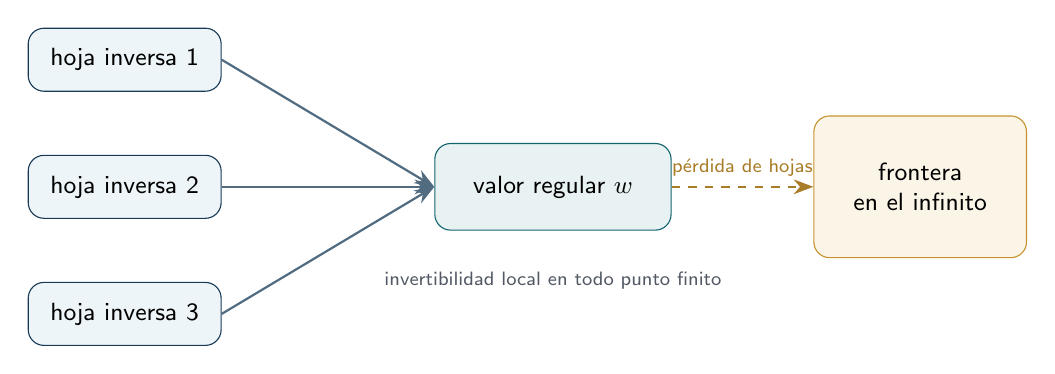
\begin{tikzpicture}[
  node distance=8mm and 15mm,
  sheet/.style={draw=deepblue,fill=softblue,rounded corners=2mm,
    minimum width=2.45cm,minimum height=8mm,font=\small\sffamily},
  target/.style={draw=teal!80!black,fill=teal!10,rounded corners=2mm,
    minimum width=3cm,minimum height=11mm,font=\small\sffamily},
  arr/.style={-{Stealth[length=2.5mm]},thick,deepblue!75}
]
\node[sheet] (s1) {hoja inversa 1};
\node[sheet,below=of s1] (s2) {hoja inversa 2};
\node[sheet,below=of s2] (s3) {hoja inversa 3};
\node[target,right=27mm of s2] (w) {valor regular $w$};
\draw[arr] (s1.east) -- (w.west);
\draw[arr] (s2.east) -- (w.west);
\draw[arr] (s3.east) -- (w.west);
\node[draw=gold,fill=softgold,rounded corners=2mm,right=18mm of w,
  minimum width=2.7cm,minimum height=18mm,font=\small\sffamily,align=center]
  (inf) {frontera\\en el infinito};
\draw[-{Stealth[length=2.5mm]},thick,gold!85!black,dashed]
  (w.east) -- node[above,font=\scriptsize\sffamily]{p\'erdida de hojas} (inf.west);
\node[below=4mm of w,font=\scriptsize\sffamily,text=paperink!75]
  {invertibilidad local en todo punto finito};
\end{tikzpicture}
\caption{El jacobiano no nulo separa localmente las ramas, pero la no
propiedad permite que hojas globales desaparezcan a trav\'es del infinito.}
\label{fig:local-global}
\end{figure}

\subsection{Estado dimensional tras el contraejemplo}

\begin{center}
\begin{tabular}{@{}cl@{}}
\toprule
Dimensi\'on & Estado \\
\midrule
$n=1$ & Verdadera: una derivada constante no nula fuerza un mapa af\'in. \\
$n=2$ & Abierta. \\
$n=3$ & Falsa por el mapa de este documento. \\
$n>3$ & Falsa por estabilizaci\'on con la identidad. \\
\bottomrule
\end{tabular}
\end{center}

\section{El mapa y el certificado m\'inimo}

Definimos $F=(F_1,F_2,F_3)\colon\C^3\to\C^3$ mediante la f\'ormula anunciada
en \cite{AlpogeAnnouncement2026} y verificada independientemente en
\cite{CounterexampleNote2026}:
\begin{align}
F_1(x,y,z)&=(1+xy)^3z+y^2(1+xy)(4+3xy),\label{eq:F1}\\
F_2(x,y,z)&=y+3x(1+xy)^2z+3xy^2(4+3xy),\label{eq:F2}\\
F_3(x,y,z)&=2x-3x^2y-x^3z.\label{eq:F3}
\end{align}

Sus grados totales son, respectivamente,
\[
(\deg F_1,\deg F_2,\deg F_3)=(7,6,4).
\]

\begin{theorem}[Certificado del contraejemplo]\label{thm:counterexample}
El mapa $F$ satisface
\[
\det JF=-2,
\]
pero no es inyectivo. En concreto,
\begin{align*}
F\left(0,0,-\frac14\right)
&=F\left(1,-\frac32,\frac{13}{2}\right)\\
&=F\left(-1,\frac32,\frac{13}{2}\right)
=\left(-\frac14,0,0\right).
\end{align*}
Por consiguiente, $F$ no tiene inversa polin\'omica.
\end{theorem}

La colisi\'on se comprueba por sustituci\'on exacta. La identidad jacobiana se
demostrar\'a en la Secci\'on~\ref{sec:structure} de una forma que evita expandir
un determinante de gran tama\~no.

\begin{remark}
El certificado es especialmente fuerte desde el punto de vista epistemol\'ogico:
no depende de estimaciones, aproximaciones num\'ericas ni una cadena extensa de
lemas. Son identidades polin\'omicas sobre $\Q$ y pueden verificarse en cualquier
sistema de \`algebra computacional o asistente formal.
\end{remark}

\subsection{Normalizaci\'on a determinante uno}

La conjetura se formula a menudo bajo la normalizaci\'on $\det JF=1$. El valor
$-2$ no representa ninguna excepci\'on sustantiva.

Una normalizaci\'on sencilla ser\'ia
\[
(F_1,F_2,-F_3/2),
\]
que conserva las colisiones y tiene determinante uno. Para evitar fracciones
en los coeficientes se puede combinar un reescalamiento del dominio y del
codominio. Definimos
\[
\widehat F(x,y,z)=
\left(
\frac12F_1(x,2y,2z),
\frac12F_2(x,2y,2z),
-\frac12F_3(x,2y,2z)
\right).
\]
Entonces
\begin{align*}
\widehat F_1&=(1+2xy)^3z+4y^2(1+2xy)(2+3xy),\\
\widehat F_2&=y+3x(1+2xy)^2z+12xy^2(2+3xy),\\
\widehat F_3&=-x+3x^2y+x^3z,
\end{align*}
y $\det J\widehat F=1$.

Esta es la versi\'on propuesta en una formalizaci\'on Lean mediante la pull
request abierta 4474 del repositorio
\texttt{google-deepmind/formal-conjectures} \cite{LezeauLean2026}. En la fecha
de esta versi\'on, la contribuci\'on a\'un no hab\'ia sido integrada ni sometida
a revisi\'on formal en el repositorio. Por ejemplo,
\[
\widehat F\left(1,-\frac34,\frac{13}{4}\right)
=
\widehat F\left(-1,\frac34,\frac{13}{4}\right)
=\left(-\frac18,0,0\right).
\]

\begin{corollary}
El contraejemplo existe sobre todo cuerpo de caracter\'istica cero.
\end{corollary}

\begin{proof}
El mapa, el determinante y los puntos de colisi\'on tienen coeficientes
racionales. Todo cuerpo de caracter\'istica cero contiene una copia de $\Q$.
\end{proof}

\clearpage
\part{Estructura algebraica y geometr\'ia global}

\section{Las variables estructurales}\label{sec:structure}

Las expresiones originales esconden una estructura mucho m\'as peque\~na.
Introducimos
\begin{equation}\label{eq:uqr}
u=1+xy,\qquad
q=u^2z+y^2(4+3xy),\qquad
r=2-3xy-x^2z.
\end{equation}

\begin{lemma}[Forma comprimida]\label{lem:compressed}
Se cumplen las identidades
\begin{equation}\label{eq:Fcompressed}
F=(uq,\;y+3xq,\;xr)
\end{equation}
y
\begin{equation}\label{eq:keyidentity}
x^2q=u+1-u^2r.
\end{equation}
\end{lemma}

\begin{proof}
La primera afirmaci\'on se obtiene directamente de
\eqref{eq:F1}--\eqref{eq:F3}. Para la segunda, usamos
$xy=u-1$ y $x^2z=5-3u-r$:
\begin{align*}
x^2q
&=u^2x^2z+x^2y^2(1+3u)\\
&=u^2(5-3u-r)+(u-1)^2(1+3u)\\
&=u+1-u^2r.
\end{align*}
\end{proof}

La identidad \eqref{eq:keyidentity} es el esqueleto algebraico del ejemplo.
En el abierto $x\neq0$, las variables originales pueden expresarse como
\[
y=\frac{u-1}{x},\qquad
z=\frac{5-3u-r}{x^2},\qquad
q=\frac{u+1-u^2r}{x^2}.
\]
Por tanto, en coordenadas $(x,u,r)$, el mapa se convierte en
\begin{equation}\label{eq:F_xur}
F(x,u,r)=
\left(
\frac{u(u+1-u^2r)}{x^2},
\frac{4u+2-3u^2r}{x},
xr
\right).
\end{equation}

\begin{proposition}[C\'alculo del jacobiano en coordenadas $(x,u,r)$]
El determinante jacobiano de $F$ es id\'enticamente $-2$.
\end{proposition}

\begin{proof}
Consideremos primero el cambio racional
\[
\Phi(x,y,z)=(x,u,r).
\]
Una diferenciaci\'on directa da
\[
\det J\Phi=-x^3.
\]
Sea $\Psi$ el mapa de \eqref{eq:F_xur}. Otro c\'alculo directo, ahora mucho m\'as
peque\~no, da
\[
\det J\Psi=\frac{2}{x^3}.
\]
En el abierto denso $x\neq0$ se tiene $F=\Psi\circ\Phi$, y por la regla de la
cadena
\[
\det JF=\frac{2}{x^3}(-x^3)=-2.
\]
Como ambos lados son polinomios, la identidad se extiende a todo $\C^3$.
\end{proof}

\begin{figure}[htbp]
\centering
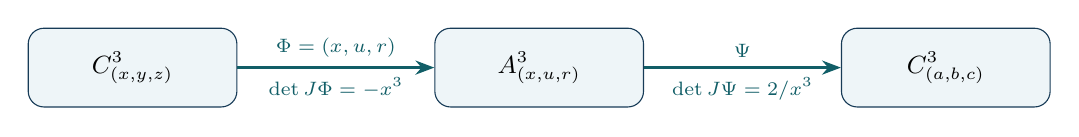
\begin{tikzpicture}[
  space/.style={draw=deepblue,fill=softblue,rounded corners=2mm,
    minimum width=2.65cm,minimum height=10mm,font=\small},
  arr/.style={-{Stealth[length=2.4mm]},thick,teal!75!black}
]
\node[space] (xyz) {$\C^3_{(x,y,z)}$};
\node[space,right=25mm of xyz] (xur) {$\A^3_{(x,u,r)}$};
\node[space,right=25mm of xur] (abc) {$\C^3_{(a,b,c)}$};
\draw[arr] (xyz)--node[above,font=\scriptsize] {$\Phi=(x,u,r)$}
  node[below,font=\scriptsize] {$\det J\Phi=-x^3$} (xur);
\draw[arr] (xur)--node[above,font=\scriptsize] {$\Psi$}
  node[below,font=\scriptsize] {$\det J\Psi=2/x^3$} (abc);
\end{tikzpicture}
\vspace{1mm}
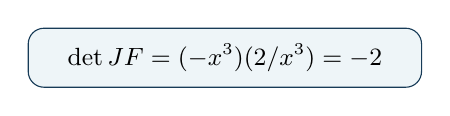
\begin{tikzpicture}
\node[draw=deepblue,fill=softblue,rounded corners=2mm,
  inner xsep=5mm,inner ysep=2mm,font=\sffamily\small]
  {$\det JF=(-x^3)(2/x^3)=-2$};
\end{tikzpicture}
\caption{Factorizaci\'on racional del mapa en las variables estructurales. La
cancelaci\'on de $x^3$ explica el jacobiano constante sin expandir un
determinante de gran tama\~no.}
\label{fig:structural-factorization}
\end{figure}

\section{La c\'ubica de las fibras}

La nota p\'ublica contempor\'anea describe las fibras mediante una incidencia
con una c\'ubica binaria \cite{CounterexampleNote2026}. Presentamos aqu\'i una
eliminaci\'on af\'in equivalente, adaptada a los c\'alculos posteriores.

Escribamos
\[
F(x,y,z)=(a,b,c)
\]
y definamos los dos polinomios del espacio de llegada
\begin{align}
D(a,b,c)&=27a^2c^2-18abc+16a+b^3c-b^2,\label{eq:D}\\
E(a,b,c)&=27ac^2-9bc+8.\label{eq:E}
\end{align}

\begin{theorem}[Ecuaci\'on de eliminaci\'on]\label{thm:cubic}
Para todo $(x,y,z)\in\C^3$, si $F(x,y,z)=(a,b,c)$, entonces
\begin{equation}\label{eq:fibercubic}
D(a,b,c)x^3+(4-3bc)x-2c=0.
\end{equation}
Sobre el cuerpo de funciones $\Q(a,b,c)$, las otras dos coordenadas se
recuperan racionalmente a partir de $x$. En particular, $F$ tiene grado
algebraico gen\'erico tres.
\end{theorem}

\begin{proof}
La identidad necesaria se verifica sustituyendo
$(a,b,c)=(F_1,F_2,F_3)$ en el lado izquierdo de
\eqref{eq:fibercubic}: el resultado se simplifica id\'enticamente a cero.

Para la afirmaci\'on gen\'erica, calculamos una base de Gr\"obner de
\[
F_1-a,\quad F_2-b,\quad F_3-c
\]
en el orden lexicogr\'afico $z>y>x$ sobre $\Q(a,b,c)$. El \'ultimo elemento es,
salvo una unidad del cuerpo de coeficientes, el polinomio c\'ubico
\eqref{eq:fibercubic}; los dos elementos anteriores son lineales en $y$ y $z$.
Tras localizar los coeficientes principales que aparecen en esas dos
ecuaciones lineales, cada ra\'iz de la c\'ubica determina de manera \'unica las
coordenadas $y$ y $z$. Rec\'iprocamente, toda preimagen proporciona una ra\'iz
por la identidad ya verificada. En el abierto adicional donde el
discriminante no se anula, la c\'ubica tiene tres ra\'ices simples; por tanto,
la fibra gen\'erica tiene tres puntos y
\[
[\Q(x,y,z):\Q(F_1,F_2,F_3)]=3.
\]
Esto justifica el paso desde la base de Gr\"obner al grado gen\'erico, y no
s\'olo la existencia de una relaci\'on c\'ubica. El c\'alculo reproducible
aparece en el Ap\'endice~\ref{app:reproducibility}.
\end{proof}

\begin{corollary}[La triple fibra explicada]
Para $(a,b,c)=(-1/4,0,0)$, la ecuaci\'on \eqref{eq:fibercubic} es
\[
-4x^3+4x=-4x(x-1)(x+1)=0.
\]
Sus tres ra\'ices $x=0,1,-1$ producen exactamente los tres puntos del
Teorema~\ref{thm:counterexample}.
\end{corollary}

Este resultado cambia la interpretaci\'on del ejemplo: no estamos ante dos
ramas que colisionan accidentalmente. Un punto gen\'erico del codominio tiene
tres preim\'agenes.

\subsection{Discriminante y grupo de Galois gen\'erico}

El discriminante respecto de $x$ de la c\'ubica \eqref{eq:fibercubic}
factoriza de forma notable:
\begin{equation}\label{eq:discriminant}
\operatorname{Disc}_x
\left(Dx^3+(4-3bc)x-2c\right)
=-4D E^2.
\end{equation}

\begin{proposition}\label{prop:S3}
La extensi\'on gen\'erica de cuerpos
\[
\C(x,y,z)/\C(F_1,F_2,F_3)
\]
tiene grado tres, no es de Galois y su cierre normal tiene grupo de Galois
$S_3$.
\end{proposition}

\begin{proof}
El grado tres procede del Teorema~\ref{thm:cubic}. Para una c\'ubica irreducible
separable, el grupo de Galois es $A_3$ si y s\'olo si el discriminante es un
cuadrado. Por \eqref{eq:discriminant}, la clase cuadr\'atica del discriminante
es la de $D$. Visto como polinomio cuadr\'atico en $a$, el discriminante de $D$
es
\[
\operatorname{Disc}_a(D)=-4(3bc-4)^3,
\]
que no es un cuadrado en $\C(b,c)$. Por tanto, $D$ es irreducible y aparece con
multiplicidad impar; en particular, no es un cuadrado en $\C(a,b,c)$. El grupo
del cierre normal es entonces $S_3$.
\end{proof}

Esto sit\'ua el contraejemplo exactamente fuera de los casos galoisianos en los
que se conoc\'ia la validez de la conjetura. La no normalidad de la extensi\'on
no es un accidente perif\'erico, sino parte del mecanismo.

\begin{figure}[htbp]
\centering
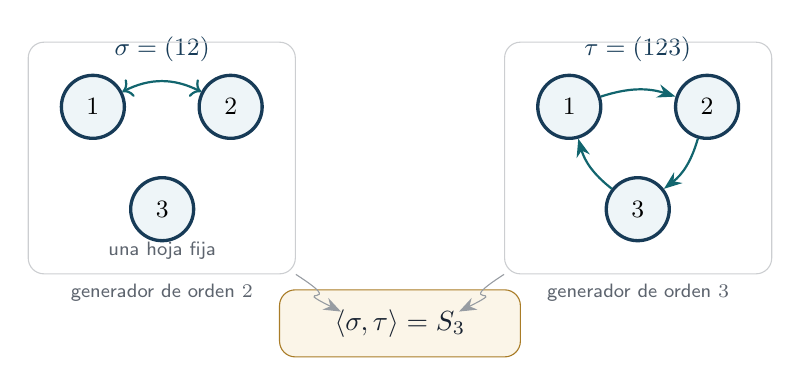
\begin{tikzpicture}[
  sheet/.style={circle,draw=deepblue,fill=softblue,very thick,
    minimum size=8mm,font=\small\sffamily\bfseries},
  panel/.style={draw=paperink!22,fill=none,rounded corners=2mm,
    inner sep=4mm},
  perm/.style={-{Stealth[length=2.3mm]},thick,teal!80!black}
]
  \node[sheet] (s1) at (-3.9,0.55) {$1$};
  \node[sheet] (s2) at (-2.15,0.55) {$2$};
  \node[sheet] (s3) at (-3.02,-0.75) {$3$};
  \draw[perm,<->,bend left=27] (s1) to (s2);
  \node[font=\small\sffamily\bfseries,text=deepblue] at (-3.02,1.28)
    {$\sigma=(12)$};
  \node[font=\scriptsize\sffamily,text=paperink!70] at (-3.02,-1.28)
    {una hoja fija};
  \node[panel,fit=(s1)(s2)(s3),label={[font=\scriptsize\sffamily,
    text=paperink!70]below:generador de orden $2$}] (p1) {};

  \node[sheet] (t1) at (2.15,0.55) {$1$};
  \node[sheet] (t2) at (3.9,0.55) {$2$};
  \node[sheet] (t3) at (3.02,-0.75) {$3$};
  \draw[perm,bend left=18] (t1) to (t2);
  \draw[perm,bend left=18] (t2) to (t3);
  \draw[perm,bend left=18] (t3) to (t1);
  \node[font=\small\sffamily\bfseries,text=deepblue] at (3.02,1.28)
    {$\tau=(123)$};
  \node[panel,fit=(t1)(t2)(t3),label={[font=\scriptsize\sffamily,
    text=paperink!70]below:generador de orden $3$}] (p2) {};

  \node[draw=gold!85!black,fill=softgold,rounded corners=2mm,
    font=\sffamily\bfseries,text=paperink,inner xsep=7mm,inner ysep=2.5mm]
    at (0,-2.2) {$\langle\sigma,\tau\rangle=S_3$};
  \draw[-{Stealth[length=2.2mm]},paperink!45] (p1.south east)
    .. controls +(0.7,-0.45) and +(-0.7,0.35) .. (-0.75,-2.05);
  \draw[-{Stealth[length=2.2mm]},paperink!45] (p2.south west)
    .. controls +(-0.7,-0.45) and +(0.7,0.35) .. (0.75,-2.05);
\end{tikzpicture}
\caption{Modelo combinatorio de la acci\'on del cierre normal sobre las tres
ramas gen\'ericas. Una transposici\'on y un ciclo de orden tres generan
$S_3$. La figura representa la acci\'on algebraica; la construcci\'on de lazos
topol\'ogicos expl\'icitos permanece abierta.}
\label{fig:s3-monodromy}
\end{figure}

\subsection{Rigidez universal en grado gen\'erico tres}

La conclusi\'on $S_3$ no es exclusiva de las f\'ormulas de este ejemplo.
Describe necesariamente a cualquier contraejemplo de grado gen\'erico tres.

\begin{theorem}[Grado gen\'erico m\'inimo y cierre normal]
\label{thm:generic-degree-three}
Sea $G\colon\C^n\to\C^n$ un mapa de Keller y escribamos
\[
d(G)=[\C(x_1,\ldots,x_n):\C(G_1,\ldots,G_n)].
\]
Si $G$ no es un automorfismo, entonces $d(G)\geq3$. La cota es \'optima por
el mapa $F$ de este documento.

Adem\'as, si $d(G)=3$ y $G$ no es un automorfismo, el cierre normal de la
extensi\'on de cuerpos tiene grupo $S_3$ y
\[
\operatorname{Aut}_{\C(G)}\C(x_1,\ldots,x_n)=\{1\}.
\]
\end{theorem}

\begin{proof}
Si $d(G)=1$, la extensi\'on es birracional y el teorema de Keller implica que
$G$ es un automorfismo. Si $d(G)=2$, la extensi\'on es separable por estar en
caracter\'istica cero y toda extensi\'on separable cuadr\'atica es de Galois;
los teoremas de Campbell--Razar--Wright vuelven a implicar que $G$ es un
automorfismo. Por tanto, un contraejemplo tiene grado gen\'erico al menos tres,
y el Teorema~\ref{thm:cubic} muestra que la cota se alcanza.

Supongamos ahora $d(G)=3$. El grupo del cierre normal act\'ua transitivamente
sobre tres hojas, de modo que es $A_3\cong C_3$ o $S_3$. En el primer caso la
extensi\'on c\'ubica ya ser\'ia normal y, por tanto, galoisiana; esto volver\'ia
a forzar que $G$ fuese un automorfismo. Luego el grupo es $S_3$. Una extensi\'on
c\'ubica no normal no posee automorfismos no triviales sobre el cuerpo base,
lo que da la \'ultima afirmaci\'on.
\end{proof}

Este teorema proporciona una primera clasificaci\'on verdadera: fija el grado
m\'inimo, el grupo de monodrom\'ia gen\'erico y la ausencia de transformaciones
de cubierta. No clasifica, sin embargo, los mapas por equivalencia polin\'omica.
La pregunta de si todo contraejemplo de grado gen\'erico tres es estable o
polin\'omicamente equivalente al presente es mucho m\'as fuerte y no se sigue
de compartir grupo $S_3$.

Para atacar esa clasificaci\'on hay que comparar al menos cuatro invariantes:
el divisor de no propiedad, su normalizaci\'on y conductor; el locus omitido;
las valuaciones del cuerpo de funciones que aparecen en el infinito; y la
representaci\'on de monodrom\'ia del complemento del discriminante. El
Teorema~\ref{thm:normalization-cusp} calcula los dos primeros para $F$ y
proporciona un modelo con el que contrastar futuros ejemplos.

\section{No propiedad y geometr\'ia en el infinito}

Un mapa propio, localmente biholomorfo $\C^3\to\C^3$ ser\'ia un recubrimiento.
Como $\C^3$ es simplemente conexo, tal recubrimiento tendr\'ia grado uno. Por
consiguiente, un mapa \`etale de grado gen\'erico tres debe perder hojas en el
infinito.

\begin{proposition}[Familia asint\'otica expl\'icita]\label{prop:asymptotic}
Fijemos $\lambda,c\in\C$ y, para $s\neq0$, pongamos
\begin{equation}\label{eq:asymcurve}
x=s,\qquad
y=\lambda-\frac1s,\qquad
z=-\frac{3\lambda}{s}+\frac5{s^2}-\frac{c}{s^3}.
\end{equation}
Entonces
\begin{equation}\label{eq:asymimage}
F(x,y,z)=
\left(
\lambda^2-\lambda^3c+\frac{\lambda}{s},
4\lambda-3\lambda^2c+\frac2s,
c
\right).
\end{equation}
En particular, cuando $|s|\to\infty$, el punto del dominio escapa al infinito
y su imagen converge a
\begin{equation}\label{eq:asym_limit}
\left(\lambda^2-\lambda^3c,\;4\lambda-3\lambda^2c,\;c\right).
\end{equation}
\end{proposition}

\begin{proof}
La sustituci\'on de \eqref{eq:asymcurve} en
\eqref{eq:F1}--\eqref{eq:F3} da exactamente \eqref{eq:asymimage}.
\end{proof}

Los l\'imites \eqref{eq:asym_limit} satisfacen
\[
D(a,b,c)=0.
\]
Por tanto, la hipersuperficie
\begin{equation}\label{eq:S}
\mathcal S=\{(a,b,c)\in\C^3:D(a,b,c)=0\}
\end{equation}
contiene una familia dominante de valores asint\'oticos. Esto exhibe de manera
concreta el lugar por el que las hojas pueden desaparecer hacia el infinito.

\begin{remark}
La triple fibra sobre $(-1/4,0,0)$ no est\'a sobre $\mathcal S$, pues all\'i
$D=-4$. Por tanto, cerca de ese valor las tres ramas inversas son regulares y
separadas. La obstrucci\'on que permite conectarlas globalmente est\'a lejos, en
la frontera asint\'otica.
\end{remark}

\subsection{La curva singular omitida}

La hipersuperficie $\mathcal S$ tiene una curva singular especialmente
significativa.

\begin{proposition}[Locus singular de la superficie asint\'otica]
El locus singular de $\mathcal S$ es
\begin{equation}\label{eq:Gamma}
\Gamma=
\left\{
\left(
\frac{4}{27c^2},\frac{4}{3c},c
\right):c\in\C^\times
\right\}.
\end{equation}
\end{proposition}

\begin{proof}
Las derivadas de $D$ son
\begin{align*}
\frac{\partial D}{\partial a}&=2(27ac^2-9bc+8)=2E,\\
\frac{\partial D}{\partial b}&=-18ac+3b^2c-2b,\\
\frac{\partial D}{\partial c}&=54a^2c-18ab+b^3.
\end{align*}
Si $c=0$, la primera derivada vale $16$, por lo que no hay puntos singulares.
Para $c\neq0$, de $E=0$ obtenemos
\[
a=\frac{9bc-8}{27c^2}.
\]
Al sustituir en $D$ resulta
\[
D=\frac{(3bc-4)^3}{27c^2}.
\]
Las ecuaciones singulares fuerzan entonces $3bc=4$ y
$27ac^2=4$, que describen exactamente \eqref{eq:Gamma}.
\end{proof}

\subsection{Normalizaci\'on y tipo de singularidad transversal}
\label{sec:normalization-cusp}

La parametrizaci\'on asint\'otica no s\'olo domina $\mathcal S$: proporciona
su normalizaci\'on. Para evitar una colisi\'on de notaci\'on con la variable
$u=1+xy$ de la Secci\'on~\ref{sec:structure}, denotamos por $\lambda$ el
par\'ametro de la normalizaci\'on y conservamos $c$ como tercera coordenada.

\begin{theorem}[Normalizaci\'on expl\'icita de $\mathcal S$]
\label{thm:normalization-cusp}
El morfismo
\begin{equation}\label{eq:normalization-map}
\nu\colon\A^2_{\lambda,c}\longrightarrow\mathcal S,
\qquad
(\lambda,c)\longmapsto
\bigl(\lambda^2-c\lambda^3,\,4\lambda-3c\lambda^2,\,c\bigr)
\end{equation}
es la normalizaci\'on de la superficie irreducible $\mathcal S$.

En el abierto $c\neq0$, pongamos
\begin{equation}\label{eq:cusp-coordinates}
h=3bc-4,\qquad E=27ac^2-9bc+8.
\end{equation}
Entonces
\begin{equation}\label{eq:cusp-identity}
E^2+h^3=27c^2D.
\end{equation}
Por tanto, en coordenadas regulares $(E,h,c)$, la superficie tiene ecuaci\'on
$E^2+h^3=0$. Su locus singular es $E=h=0$, es decir, $\Gamma$, y una secci\'on
transversal a $\Gamma$ es la c\'uspide ordinaria $X^2+Y^3=0$.
\end{theorem}

\begin{proof}
La sustituci\'on de \eqref{eq:normalization-map} en $D$ da cero. Adem\'as,
$D$ es irreducible: visto como polinomio cuadr\'atico primitivo en $a$ sobre
$\C[b,c]$, su discriminante es
\[
\operatorname{Disc}_a(D)=-4(3bc-4)^3,
\]
que no es un cuadrado en $\C(b,c)$. Por ello la imagen de $\nu$ es densa en
$\mathcal S$.

En el anillo de coordenadas de $\mathcal S$, el elemento $\lambda$ satisface
la ecuaci\'on m\'onica
\begin{equation}\label{eq:normalization-integral}
\lambda^2-b\lambda+3a=0.
\end{equation}
La extensi\'on inducida
$\C[a,b,c]/(D)\hookrightarrow\C[\lambda,c]$ es integral. Es tambi\'en
birracional, porque en el abierto $4-3bc\neq0$ se recupera el par\'ametro por
\begin{equation}\label{eq:normalization-birational}
\lambda=\frac{b-9ac}{4-3bc}.
\end{equation}
Como $\C[\lambda,c]$ es normal, \eqref{eq:normalization-map} es la
normalizaci\'on.

La identidad \eqref{eq:cusp-identity} se verifica por expansi\'on directa. El
cambio $(a,b,c)\mapsto(E,h,c)$ es invertible cuando $c\neq0$, pues
\[
b=\frac{h+4}{3c},\qquad a=\frac{E+3h+4}{27c^2}.
\]
As\'i, $\mathcal S$ es localmente el producto de la c\'uspide plana con la
coordenada suave $c$.
\end{proof}

Si $v=3c\lambda-2$, entonces
\begin{equation}\label{eq:cusp-pullback}
\nu^*h=-v^2,\qquad \nu^*E=-v^3.
\end{equation}
En el abierto $c\neq0$, el ideal conductor es $(E,h)$ en la superficie y
$(v^2)$ en su normalizaci\'on. La preimagen de $\Gamma$ es la curva lisa
$v=0$. Esto explica simult\'aneamente la no normalidad de $\mathcal S$, la
singularidad de su discriminante y la aparici\'on de la curva omitida.

En efecto, despu\'es de invertir $c$ y mediante las coordenadas regulares
anteriores, la inclusi\'on de anillos toma la forma
\[
R[v^2,v^3]\subset R[v],\qquad R=\C[c,c^{-1}],
\]
con $h=-v^2$ y $E=-v^3$. El mayor ideal de $R[v]$ contenido en
$R[v^2,v^3]$ es $v^2R[v]$: todos sus monomios tienen exponente al menos dos y
pertenecen al subanillo, mientras que ning\'un elemento de orden $0$ o $1$ en
$v$ puede multiplicar todo $R[v]$ dentro del subanillo. Su contracci\'on es
$(v^2,v^3)=(h,E)$. Esta identificaci\'on demuestra, y no s\'olo anuncia, las
dos expresiones del conductor usadas en la figura siguiente.

\begin{figure}[htbp]
\centering
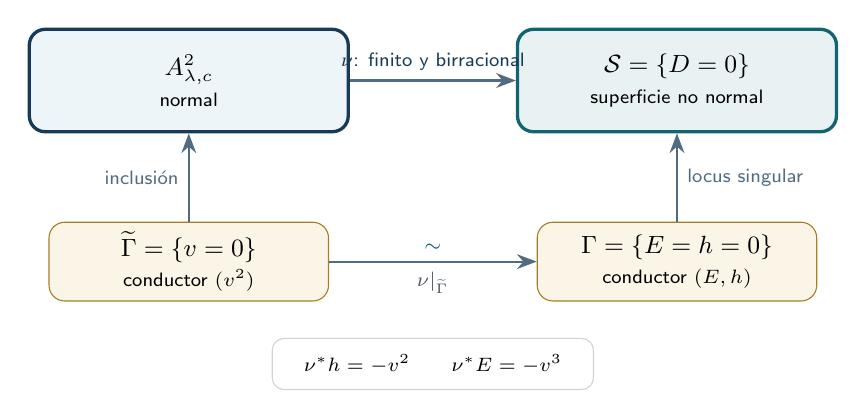
\begin{tikzpicture}[
  space/.style={draw=deepblue,fill=softblue,very thick,rounded corners=2mm,
    minimum width=4.05cm,minimum height=13mm,align=center,font=\small\sffamily},
  singular/.style={draw=teal!80!black,fill=teal!10,very thick,
    rounded corners=2mm,minimum width=4.05cm,minimum height=13mm,
    align=center,font=\small\sffamily},
  curve/.style={draw=gold!85!black,fill=softgold,rounded corners=2mm,
    minimum width=3.55cm,minimum height=10mm,align=center,font=\small\sffamily},
  arr/.style={-{Stealth[length=2.5mm]},thick,deepblue!75}
]
  \node[space] (normal) at (-3.1,1.15)
    {$\A^2_{\lambda,c}$\\\scriptsize normal};
  \node[singular] (surface) at (3.1,1.15)
    {$\mathcal S=\{D=0\}$\\\scriptsize superficie no normal};
  \draw[arr] (normal) -- node[above,font=\scriptsize\sffamily,
    text=deepblue] {$\nu$: finito y birracional} (surface);

  \node[curve] (pre) at (-3.1,-1.15)
    {$\widetilde\Gamma=\{v=0\}$\\\scriptsize conductor $(v^2)$};
  \node[curve] (gamma) at (3.1,-1.15)
    {$\Gamma=\{E=h=0\}$\\\scriptsize conductor $(E,h)$};
  \draw[arr] (pre) -- node[below,font=\scriptsize\sffamily,
    text=paperink!75] {$\nu|_{\widetilde\Gamma}$} node[above,
    font=\scriptsize\sffamily,text=teal!75!black] {$\sim$} (gamma);
  \draw[arr] (pre) -- node[left,font=\scriptsize\sffamily] {inclusi\'on}
    (normal);
  \draw[arr] (gamma) -- node[right,font=\scriptsize\sffamily] {locus singular}
    (surface);

  \node[draw=paperink!20,fill=white,rounded corners=1.5mm,
    font=\scriptsize\sffamily,align=center,inner xsep=4mm,inner ysep=2mm]
    at (0,-2.45) {$\nu^*h=-v^2$\qquad $\nu^*E=-v^3$};
\end{tikzpicture}
\caption{Diagrama global de la normalizaci\'on y del conductor. La curva lisa
$\widetilde\Gamma$ de la normalizaci\'on se identifica con la curva singular
$\Gamma$, mientras que las potencias $v^2$ y $v^3$ producen la c\'uspide
transversal.}
\label{fig:global-normalization}
\end{figure}

\begin{figure}[htbp]
\centering
\begin{tikzpicture}[scale=1.05]
  \draw[-{Stealth[length=2mm]},paperink!65] (-3.2,0)--(1.0,0)
    node[right,font=\scriptsize] {$h$};
  \draw[-{Stealth[length=2mm]},paperink!65] (0,-2.25)--(0,2.25)
    node[above,font=\scriptsize] {$E$};
  \draw[very thick,teal,domain=-1.45:1.45,samples=90,smooth,variable=\t]
    plot ({-1.35*\t*\t},{1.05*\t*\t*\t});
  \fill[gold] (0,0) circle (2.3pt);
  \node[font=\scriptsize\sffamily,align=left,anchor=west] at (1.15,1.25)
    {$h=-v^2$\\$E=-v^3$};
  \draw[-{Stealth[length=2mm]},deepblue,dashed]
    (1.15,0.95) .. controls +(0,-0.5) and +(0.6,0.5) .. (-0.55,-0.35);
  \node[font=\scriptsize\sffamily,below right=1mm and 1mm] at (0,0)
    {$\Gamma$};
\end{tikzpicture}
\caption{Secci\'on transversal de la superficie asint\'otica. La
normalizaci\'on $v\mapsto(h,E)=(-v^2,-v^3)$ resuelve la c\'uspide y env\'ia
$v=0$ a la curva omitida $\Gamma$.}
\label{fig:cusp-normalization}
\end{figure}

\begin{theorem}[Una curva fuera de la imagen]\label{thm:omitted}
Ning\'un punto de $\Gamma$ pertenece a la imagen de $F$.
\end{theorem}

\begin{proof}
Para un punto de $\Gamma$ se tiene
\[
D=0,\qquad 4-3bc=0,
\]
mientras que $c\neq0$. La ecuaci\'on necesaria de la fibra
\eqref{eq:fibercubic} se reduce a
\[
-2c=0,
\]
una contradicci\'on.
\end{proof}

\begin{corollary}
El mapa $F$ no es sobreyectivo.
\end{corollary}

La curva omitida es, simult\'aneamente, el locus singular de la superficie de
valores asint\'oticos. Esta coincidencia permite cerrar por completo la
descripci\'on de la imagen; una descripci\'on equivalente mediante ra\'ices
simples de la c\'ubica binaria aparece en \cite{CounterexampleNote2026}.

\begin{theorem}[Imagen exacta]\label{thm:exact-image}
Se tiene
\[
F(\C^3)=\C^3\setminus\Gamma.
\]
\end{theorem}

\begin{proof}
El Teorema~\ref{thm:omitted} prueba una de las inclusiones. Fijemos ahora
$(a,b,c)\notin\Gamma$ y escribamos
\[
P_{a,b,c}(X)=D(a,b,c)X^3+(4-3bc)X-2c.
\]
Si $c=0$, existe la preimagen expl\'icita
\[
F\bigl(0,b,a-4b^2\bigr)=(a,b,0).
\]
Supongamos $c\neq0$. Si $a=0$ y $b=0$, entonces
\[
F\left(\frac c2,0,0\right)=(0,0,c),
\]
mientras que, si $a=0$ y $b\neq0$,
\[
F\left(\frac2b,-\frac b2,\frac{b^2(10-bc)}8\right)=(0,b,c).
\]

Queda el caso $ac\neq0$. Fuera de $\Gamma$, el polinomio $P_{a,b,c}$ no puede
ser una constante no nula. En efecto, si $D=0$ y $3bc=4$, entonces
\[
D=\frac{(27ac^2-4)^2}{27c^2},
\]
y la anulaci\'on de $D$ situar\'ia $(a,b,c)$ en $\Gamma$. Por tanto,
$P_{a,b,c}$ tiene una ra\'iz $x\in\C$; como $c\neq0$, se tiene $x\neq0$.

Consideremos
\begin{align*}
R_1(U)&=U^2-(1+bx)U+3ax^2,\\
R_2(U)&=cU^3-xU(U+1)+ax^3.
\end{align*}
El c\'alculo de la resultante da
\begin{equation}\label{eq:resultant-u}
\operatorname{Res}_U(R_1,R_2)=ax^3P_{a,b,c}(x)=0.
\end{equation}
As\'i, $R_1$ y $R_2$ tienen una ra\'iz com\'un $u$, necesariamente no nula
porque $R_1(0)=3ax^2\neq0$. Definimos
\[
q=\frac au,\qquad
y=b-3xq,\qquad
r=\frac cx,\qquad
z=\frac{2-3xy-r}{x^2}.
\]
La ecuaci\'on $R_1(u)=0$ equivale a $u=1+xy$, y $R_2(u)=0$ equivale a
\[
x^2q=u+1-u^2r.
\]
El Lema~\ref{lem:compressed} implica entonces $F(x,y,z)=(a,b,c)$.
\end{proof}

\subsection{Determinaci\'on exacta del conjunto de no propiedad}

Denotemos por $\mathcal N_F$ el conjunto de valores $w$ para los que existe
una sucesi\'on $p_\nu\in\C^3$ con
$\lVert p_\nu\rVert\to\infty$ y $F(p_\nu)\to w$. Esta es la noci\'on cl\'asica
de conjunto de no propiedad \cite{Jelonek1993}; para este mapa, su
determinaci\'on tambi\'en se obtiene en \cite{CounterexampleNote2026}.

\begin{theorem}[Conjunto exacto de no propiedad]\label{thm:nonproperness}
Se tiene
\[
\mathcal N_F=\mathcal S=\{D=0\}.
\]
\end{theorem}

\begin{proof}
Probemos primero $\mathcal S\subseteq\mathcal N_F$. Si
$(a,b,0)\in\mathcal S$, entonces $16a-b^2=0$ y, tomando
$\lambda=b/4$, se obtiene $(a,b,0)=(\lambda^2,4\lambda,0)$. Si $c\neq0$, los
polinomios
\[
a-\lambda^2(1-\lambda c),
\qquad
b-\lambda(4-3\lambda c)
\]
tienen resultante $cD(a,b,c)$ respecto de $\lambda$. Cuando $D=0$ poseen una
ra\'iz com\'un. En ambos casos, la familia de la
Proposici\'on~\ref{prop:asymptotic} converge a $(a,b,c)$ desde el infinito.

Para la inclusi\'on contraria, sea
$p_\nu=(x_\nu,y_\nu,z_\nu)$ una sucesi\'on no acotada tal que
\[
F(p_\nu)=(A_\nu,B_\nu,C_\nu)\longrightarrow(a,b,c),
\]
y pongamos $u_\nu=1+x_\nu y_\nu$. Las identidades estructurales dan
\begin{equation}\label{eq:u-bounded}
u_\nu^2-(1+B_\nu x_\nu)u_\nu+3A_\nu x_\nu^2=0.
\end{equation}
Si $(x_\nu)$ fuese acotada, tambi\'en lo ser\'ia $(u_\nu)$. Si
$x_\nu\to x_0\neq0$, las f\'ormulas
\[
y_\nu=\frac{u_\nu-1}{x_\nu},\qquad
r_\nu=\frac{C_\nu}{x_\nu},\qquad
z_\nu=\frac{5-3u_\nu-r_\nu}{x_\nu^2}
\]
har\'ian acotada toda la sucesi\'on, una contradicci\'on.

Supongamos $x_\nu\to0$. Si $u_\nu\to0$ en alguna subsucesi\'on,
\eqref{eq:u-bounded} da $u_\nu=O(x_\nu^2)$. Pero
\begin{align*}
x_\nu B_\nu
&=(u_\nu-1)+3x_\nu^2q_\nu\\
&=(u_\nu-1)+3(u_\nu+1-u_\nu^2r_\nu),
\end{align*}
con $r_\nu=C_\nu/x_\nu$; el lado derecho tender\'ia a $2$ y el izquierdo a
$0$. Por tanto, $u_\nu$ permanece separado de cero. Entonces
$q_\nu=A_\nu/u_\nu$ y $y_\nu=B_\nu-3x_\nu q_\nu$ son acotados,
$u_\nu\to1$, y
\[
z_\nu=\frac{q_\nu-y_\nu^2(1+3u_\nu)}{u_\nu^2}
\]
tambi\'en es acotado. Esta contradicci\'on demuestra que toda sucesi\'on
asint\'otica tiene una subsucesi\'on con $|x_\nu|\to\infty$.

Dividiendo la ecuaci\'on de la fibra por $x_\nu^3$ obtenemos
\[
D(A_\nu,B_\nu,C_\nu)
+\frac{4-3B_\nu C_\nu}{x_\nu^2}
-\frac{2C_\nu}{x_\nu^3}=0.
\]
Al tomar l\'imites resulta $D(a,b,c)=0$, y por tanto
$\mathcal N_F\subseteq\mathcal S$.
\end{proof}

\subsection{Estratificaci\'on global de las fibras}

Los teoremas anteriores completan la geometr\'ia b\'asica del mapa.

\begin{theorem}[Cardinalidad de todas las fibras]\label{thm:fiber-strata}
Para $w\in\C^3$ se tiene
\[
\#F^{-1}(w)=
\begin{cases}
3,&w\notin\mathcal S,\\
1,&w\in\mathcal S\setminus\Gamma,\\
0,&w\in\Gamma.
\end{cases}
\]
Todas las preim\'agenes son reducidas.
\end{theorem}

\begin{proof}
Sobre $\C^3\setminus\mathcal S$, el
Teorema~\ref{thm:nonproperness} muestra que $F$ es propio. Como adem\'as es
\`etale, su restricci\'on es una cubierta finita no ramificada. El abierto
$\C^3\setminus\mathcal S$ es irreducible y el grado gen\'erico es tres, por lo
que todas sus fibras tienen tres puntos.

Si $w=(a,b,c)\in\mathcal S\setminus\Gamma$, entonces $D=0$ y
$4-3bc\neq0$; la ecuaci\'on \eqref{eq:fibercubic} determina una \'unica
coordenada $x$. Adem\'as $E\neq0$, pues $D=E=0$ describe exactamente
$\Gamma$. La base de Gr\"obner localizada en $E$ recupera de manera \'unica
$y$ y $z$. El Teorema~\ref{thm:exact-image} garantiza que esa preimagen
existe. Sobre $\Gamma$ no hay preim\'agenes por el
Teorema~\ref{thm:omitted}. Finalmente, $\det JF=-2$ garantiza que toda
preimagen finita es reducida.
\end{proof}

Sobre el abierto de tres hojas, la monodrom\'ia gen\'erica es $S_3$ por la
Proposici\'on~\ref{prop:S3}. Al alcanzar
$\mathcal S\setminus\Gamma$, dos hojas escapan al infinito y queda una sola
preimagen. Sobre el locus singular $\Gamma$ tambi\'en desaparece la tercera.
Esta es una descripci\'on global y exacta del mecanismo local--global que
destruye la conjetura.

\begin{figure}[htbp]
\centering
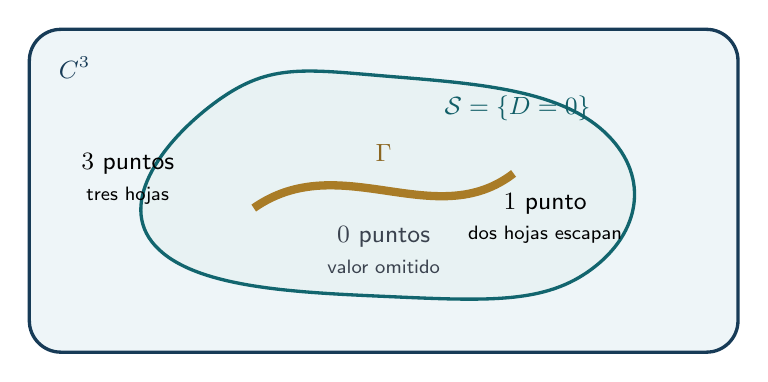
\begin{tikzpicture}[font=\small\sffamily]
  \draw[deepblue,very thick,rounded corners=4mm,fill=softblue]
    (-4.5,-2.05) rectangle (4.5,2.05);
  \node[anchor=north west,text=deepblue] at (-4.25,1.82)
    {$\C^3$};
  \draw[teal!80!black,very thick,fill=teal!10]
    plot[smooth cycle,tension=0.8] coordinates
    {(-2.9,-0.7) (-2.1,1.15) (0.1,1.45) (2.8,0.75)
     (2.7,-0.95) (0.2,-1.35)};
  \node[text=teal!75!black] at (1.7,1.05) {$\mathcal S=\{D=0\}$};
  \draw[gold!85!black,line width=3pt]
    (-1.65,-0.22) .. controls (-0.55,0.55) and (0.65,-0.55) .. (1.65,0.22);
  \node[text=gold!70!black,above] at (0,0.25) {$\Gamma$};
  \node[align=center] at (-3.25,0.15)
    {$3$ puntos\\\scriptsize tres hojas};
  \node[align=center] at (2.05,-0.35)
    {$1$ punto\\\scriptsize dos hojas escapan};
  \node[align=center,text=paperink!85] at (0,-0.75)
    {$0$ puntos\\\scriptsize valor omitido};
\end{tikzpicture}
\caption{Estratificaci\'on exacta del codominio por cardinalidad de fibra:
$3$ fuera de $\mathcal S$, $1$ sobre $\mathcal S\setminus\Gamma$ y $0$ sobre
$\Gamma$.}
\label{fig:fiber-stratification}
\end{figure}

\clearpage
\part{Grados superiores y formas normales}

\section{El fen\'omeno cu\'artico: omisi\'on y singularidad se separan}
\label{sec:quartic}

La igualdad
\[
\C^3\setminus F(\C^3)=\Sing(\mathcal N_F)
\]
es una caracter\'istica llamativa del ejemplo c\'ubico: la curva omitida
$\Gamma$ coincide con el locus singular de la hipersuperficie de no
propiedad. En esta secci\'on demostramos que esa coincidencia no persiste en
una especializaci\'on cu\'artica de la familia de mapas de Keller construida en
\cite{CounterexampleNote2026}.

Pongamos
\begin{equation}\label{eq:quartic-ab}
\alpha=1+xy,\qquad
\beta=\alpha^2z+y^2(4+3xy)
\end{equation}
y
\[
P=\alpha\beta,\qquad
Q=y+3x\beta,\qquad
R=2x-3x^2y-x^3z.
\]
Definimos el mapa polin\'omico
\begin{equation}\label{eq:F4}
F_4=(P,Q_4,R_4)\colon\C^3\longrightarrow\C^3,
\end{equation}
donde
\begin{equation}\label{eq:F4-coordinates}
Q_4=Q+\alpha^2x^2\beta^4,
\qquad
R_4=R-\frac12x^4\beta^4.
\end{equation}

\begin{proposition}[Modelo cu\'artico de las fibras]\label{prop:quartic-model}
El mapa $F_4$ satisface
\[
\det JF_4=-2.
\]
Si $F_4(x,y,z)=(p,q,r)$ y $p\neq0$, sus preim\'agenes est\'an en biyecci\'on
con las ra\'ices simples de
\begin{equation}\label{eq:quartic-fiber}
\Omega_{p,q,r}(S)
=\frac12p^4S^4+2pS^3-qS^2+2S-r.
\end{equation}
Para una ra\'iz simple $s$, la preimagen correspondiente viene dada por
\begin{equation}\label{eq:quartic-reconstruction}
\begin{split}
y&=q-3ps-p^4s^2,\qquad D=1-sy=\frac12\Omega'_{p,q,r}(s),\\
x&=\frac{s}{D},\qquad
z=pD^3-y^2(4-sy)D.
\end{split}
\end{equation}
En particular, el grado gen\'erico de $F_4$ es cuatro.
\end{proposition}

\begin{proof}
Trabajemos primero en el abierto $\alpha\neq0$ y pongamos $s=x/\alpha$.
En las coordenadas $(P,y,s)$, las dos componentes restantes son
\begin{align*}
Q_4&=y+\varphi(P,s),
&\varphi(p,s)&=3ps+p^4s^2,\\
R_4&=2s-ys^2-\vartheta(P,s),
&\vartheta(p,s)&=ps^3+\frac12p^4s^4.
\end{align*}
La identidad
\[
\frac{\partial\vartheta}{\partial s}
=s^2\frac{\partial\varphi}{\partial s}
\]
da
\[
\det\frac{\partial(P,Q_4,R_4)}{\partial(P,y,s)}
=2(1-sy).
\]
Por otro lado,
\[
\det\frac{\partial(P,y,s)}{\partial(x,y,z)}=-\alpha,
\qquad
1-sy=\frac1\alpha.
\]
La regla de la cadena produce $\det JF_4=-2$ sobre $\alpha\neq0$; como se
trata de una identidad polin\'omica, vale en todo $\C^3$.

Al eliminar
$y=q-3ps-p^4s^2$ de la ecuaci\'on de $R_4$ se obtiene exactamente
\eqref{eq:quartic-fiber}. Adem\'as,
\begin{equation}\label{eq:quartic-derivative}
\Omega'_{p,q,r}(s)
=2\bigl(1-s(q-3ps-p^4s^2)\bigr)=2D.
\end{equation}
Si $p\neq0$, toda preimagen satisface $\alpha\neq0$, porque
$p=P=\alpha\beta$. Por consiguiente $D=1/\alpha\neq0$, y la ra\'iz asociada
es simple. Rec\'iprocamente, si $s$ es simple, entonces $D\neq0$ y una
sustituci\'on directa en \eqref{eq:quartic-ab}--\eqref{eq:F4-coordinates}
prueba que las f\'ormulas \eqref{eq:quartic-reconstruction} definen una
preimagen. La cu\'artica tiene coeficiente principal $p^4/2\neq0$, de modo que
un punto general posee cuatro ra\'ices simples y, por tanto, cuatro
preim\'agenes.
\end{proof}

Sea
\[
\Delta_4(p,q,r)=\operatorname{Disc}_S\Omega_{p,q,r}(S)
\]
y denotemos por $\mathcal N_4$ el conjunto de no propiedad de $F_4$.

\begin{proposition}[No propiedad sobre $p\neq0$]
\label{prop:quartic-nonproperness}
En el abierto $U=\{p\neq0\}$ se tiene
\[
\mathcal N_4\cap U=V(\Delta_4)\cap U.
\]
\end{proposition}

\begin{proof}
Supongamos primero que $\Omega_{p,q,r}$ tiene una ra\'iz m\'ultiple $t$.
La identidad \eqref{eq:quartic-derivative} muestra que $t\neq0$ y que
\begin{equation}\label{eq:quartic-multiple-root}
q=\frac1t+3pt+p^4t^2,
\qquad
r=t-pt^3-\frac12p^4t^4.
\end{equation}
Para $\varepsilon\neq0$, definamos
\begin{equation}\label{eq:quartic-asymptotic-general}
\begin{aligned}
x_\varepsilon&=\frac{t}{\varepsilon},
&y_\varepsilon&=\frac{1-\varepsilon}{t},\\
z_\varepsilon&=p\varepsilon^3
-y_\varepsilon^2(4-ty_\varepsilon)\varepsilon.
\end{aligned}
\end{equation}
Entonces $\alpha=1/\varepsilon$, $\beta=p\varepsilon$ y una sustituci\'on
exacta da
\begin{equation}\label{eq:quartic-asymptotic-image}
F_4(x_\varepsilon,y_\varepsilon,z_\varepsilon)
=\left(p,q-\frac{\varepsilon}{t},r+\varepsilon t\right).
\end{equation}
El dominio escapa al infinito mientras la imagen converge a $(p,q,r)$.
Esto prueba
$V(\Delta_4)\cap U\subseteq\mathcal N_4\cap U$.

Para la inclusi\'on contraria, sea $K$ un compacto contenido en
$U\setminus V(\Delta_4)$. Los coeficientes principales de las cu\'articas
\eqref{eq:quartic-fiber} permanecen separados de cero, por lo que todas sus
ra\'ices quedan en un disco fijo. El conjunto de pares
\[
\{((p,q,r),s):(p,q,r)\in K,\ \Omega_{p,q,r}(s)=0\}
\]
es compacto. En \'el, $\Omega'$ no se anula; por compacidad, $|D|=|\Omega'|/2$
queda separado de cero. Las f\'ormulas
\eqref{eq:quartic-reconstruction} acotan entonces uniformemente $x,y,z$.
As\'i, $F_4^{-1}(K)$ es cerrado y acotado, luego compacto. Por tanto, no hay
valores de no propiedad fuera del discriminante.
\end{proof}

Para hablar del locus singular usamos la estructura reducida. El c\'alculo
exacto del discriminante da
\begin{equation}\label{eq:quartic-discriminant-factor}
\Delta_4=-4p^2H(p,q,r),
\end{equation}
donde $H$ es libre de cuadrados. El Ap\'endice~\ref{app:reproducibility}
incluye el c\'alculo de $H$ y la verificaci\'on
\[
\gcd(H,H_p,H_q,H_r)=1.
\]
Por tanto, sobre $U$ la ecuaci\'on reducida de $\mathcal N_4$ es $H=0$.

\begin{theorem}[Separaci\'on entre omisi\'on y singularidad]
\label{thm:quartic-separation}
Sea
\[
\mathcal E_4=\C^3\setminus F_4(\C^3).
\]
Entonces
\begin{equation}\label{eq:quartic-strict-inclusion}
\mathcal E_4\cap U
\subsetneq
\Sing(\mathcal N_4)\cap U.
\end{equation}
En particular,
\[
\mathcal E_4\neq\Sing(\mathcal N_4).
\]
\end{theorem}

\begin{proof}
Por la Proposici\'on~\ref{prop:quartic-model}, un punto de $U$ es omitido si
y s\'olo si su cu\'artica no tiene ninguna ra\'iz simple. Sus multiplicidades
son entonces de tipo $2+2$ o $4$. En ambos casos
$\Omega$ y $\Omega'$ tienen un m\'aximo com\'un divisor de grado al menos dos.
La matriz de Sylvester que define
$\operatorname{Res}(\Omega,\Omega')$ tiene, por tanto, corango al menos dos.
La diferencial del determinante de una matriz de corango al menos dos es
cero, pues su adjunta se anula. En consecuencia, todas las primeras derivadas
del discriminante se anulan. Como $H$ es una ecuaci\'on reducida sobre $U$,
esto prueba
\[
\mathcal E_4\cap U\subseteq\Sing(\mathcal N_4)\cap U.
\]

La inclusi\'on es estricta. Consideremos
\begin{equation}\label{eq:quartic-b}
b=\left(1,\frac{15}{4},\frac{11}{32}\right).
\end{equation}
Su cu\'artica factoriza como
\begin{equation}\label{eq:quartic-b-factor}
\Omega_b(S)
=\frac12\left(S-\frac12\right)^3
\left(S+\frac{11}{2}\right).
\end{equation}
La ra\'iz triple hace singular el discriminante por el mismo argumento de la
matriz de Sylvester. La ra\'iz simple $s=-11/2$, en cambio, produce mediante
\eqref{eq:quartic-reconstruction} la preimagen racional
\begin{equation}\label{eq:quartic-b-preimage}
F_4\left(\frac{11}{108},-10,-432864\right)
=\left(1,\frac{15}{4},\frac{11}{32}\right).
\end{equation}
As\'i,
$b\in\Sing(\mathcal N_4)\setminus\mathcal E_4$.

Para exhibir adem\'as un punto realmente omitido, tomemos
\begin{equation}\label{eq:quartic-c}
c=\left(2,-\frac{17}{2},-2\right).
\end{equation}
Entonces
\begin{equation}\label{eq:quartic-c-factor}
\Omega_c(S)
=8\left(S^2+\frac14S+\frac12\right)^2.
\end{equation}
No hay ra\'ices simples y $p=2\neq0$; por tanto, $c\in\mathcal E_4$.
\end{proof}

\begin{corollary}[Estratificaci\'on cu\'artica sobre $p\neq0$]
\label{cor:quartic-strata}
La cardinalidad de una fibra de $F_4$ sobre $U$ es el n\'umero de ra\'ices
simples de $\Omega$. En funci\'on de la partici\'on de multiplicidades se tiene
\[
\begin{array}{c|ccccc}
\text{tipo de ra\'ices}&1+1+1+1&2+1+1&3+1&2+2&4\\
\hline
\#F_4^{-1}(p,q,r)&4&2&1&0&0.
\end{array}
\]
El tipo $3+1$ explica exactamente el fallo de la coincidencia c\'ubica: el
discriminante ya es singular, pero todav\'ia sobrevive una rama inversa.
\end{corollary}

\begin{figure}[htbp]
\centering
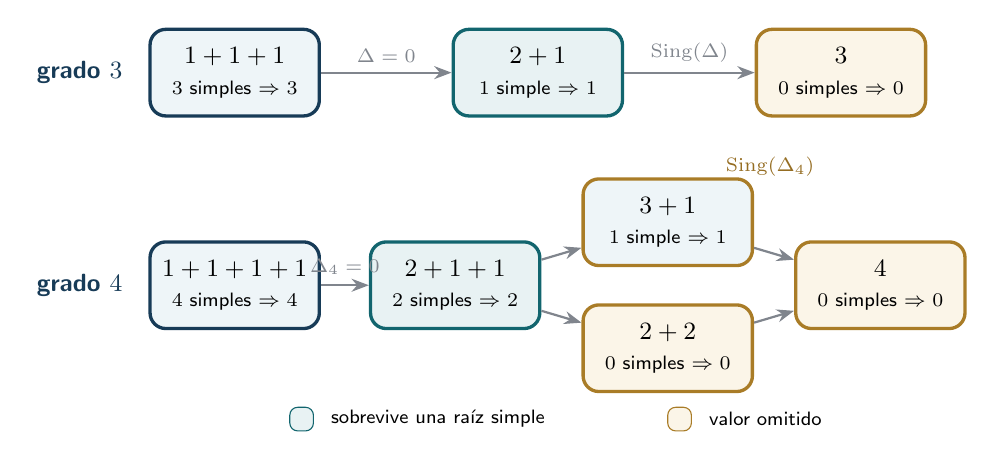
\begin{tikzpicture}[
  generic/.style={draw=deepblue,fill=softblue,very thick,rounded corners=2mm,
    minimum width=2.15cm,minimum height=11mm,align=center,font=\small\sffamily},
  boundary/.style={draw=teal!80!black,fill=teal!10,very thick,
    rounded corners=2mm,minimum width=2.15cm,minimum height=11mm,
    align=center,font=\small\sffamily},
  survive/.style={draw=gold!85!black,fill=softblue,very thick,
    rounded corners=2mm,minimum width=2.15cm,minimum height=11mm,
    align=center,font=\small\sffamily},
  omitted/.style={draw=gold!85!black,fill=softgold,very thick,
    rounded corners=2mm,minimum width=2.15cm,minimum height=11mm,
    align=center,font=\small\sffamily},
  arr/.style={-{Stealth[length=2.2mm]},thick,paperink!55}
]
  \node[font=\small\sffamily\bfseries,text=deepblue,anchor=east]
    at (-5.15,2.05) {grado $3$};
  \node[generic] (c111) at (-3.85,2.05)
    {$1+1+1$\\\scriptsize $3$ simples $\Rightarrow3$};
  \node[boundary] (c21) at (0,2.05)
    {$2+1$\\\scriptsize $1$ simple $\Rightarrow1$};
  \node[omitted] (c3) at (3.85,2.05)
    {$3$\\\scriptsize $0$ simples $\Rightarrow0$};
  \draw[arr] (c111) -- node[above,font=\scriptsize\sffamily]
    {$\Delta=0$} (c21);
  \draw[arr] (c21) -- node[above,font=\scriptsize\sffamily]
    {$\Sing(\Delta)$} (c3);

  \node[font=\small\sffamily\bfseries,text=deepblue,anchor=east]
    at (-5.15,-0.65) {grado $4$};
  \node[generic] (q1111) at (-3.85,-0.65)
    {$1+1+1+1$\\\scriptsize $4$ simples $\Rightarrow4$};
  \node[boundary] (q211) at (-1.05,-0.65)
    {$2+1+1$\\\scriptsize $2$ simples $\Rightarrow2$};
  \node[survive] (q31) at (1.65,0.15)
    {$3+1$\\\scriptsize $1$ simple $\Rightarrow1$};
  \node[omitted] (q22) at (1.65,-1.45)
    {$2+2$\\\scriptsize $0$ simples $\Rightarrow0$};
  \node[omitted] (q4) at (4.35,-0.65)
    {$4$\\\scriptsize $0$ simples $\Rightarrow0$};
  \draw[arr] (q1111) -- node[above,font=\scriptsize\sffamily]
    {$\Delta_4=0$} (q211);
  \draw[arr] (q211) -- (q31);
  \draw[arr] (q211) -- (q22);
  \draw[arr] (q31) -- (q4);
  \draw[arr] (q22) -- (q4);
  \node[font=\scriptsize\sffamily\bfseries,text=gold!75!black]
    at (2.95,0.85) {$\Sing(\Delta_4)$};

  \node[draw=teal!80!black,fill=teal!10,rounded corners=1mm,
    minimum width=3mm,minimum height=3mm] at (-3.0,-2.35) {};
  \node[anchor=west,font=\scriptsize\sffamily] at (-2.75,-2.35)
    {sobrevive una ra\'iz simple};
  \node[draw=gold!85!black,fill=softgold,rounded corners=1mm,
    minimum width=3mm,minimum height=3mm] at (1.8,-2.35) {};
  \node[anchor=west,font=\scriptsize\sffamily] at (2.05,-2.35)
    {valor omitido};
\end{tikzpicture}
\caption{Atlas de particiones de multiplicidad. La cardinalidad de la fibra
es el n\'umero de partes iguales a $1$. En grado tres, singularidad del
discriminante y omisi\'on coinciden; en grado cuatro, el estrato $3+1$ conserva
una preimagen y separa ambos fen\'omenos.}
\label{fig:multiplicity-atlas}
\end{figure}

\section{Consecuencias por dimensi\'on y grado}

\subsection{Estabilizaci\'on}

Para $n>3$, definimos
\[
F^{(n)}(x_1,\ldots,x_n)=
\bigl(F(x_1,x_2,x_3),x_4,\ldots,x_n\bigr).
\]
Entonces
\[
\det JF^{(n)}=-2
\]
y las colisiones de $F$ persisten. Por tanto, la conjetura es falsa en toda
dimensi\'on $n\geq3$.

\subsection{Grado m\'inimo}

Wang demostr\'o la conjetura para mapas de grado total a lo sumo dos
\cite{Wang1980}. El ejemplo presente tiene grado m\'aximo siete. En dimensi\'on
tres obtenemos, por tanto, el intervalo inicial
\[
3\leq d_{\min}\leq7
\]
para el menor grado posible de un contraejemplo. Determinar $d_{\min}$ es una
pregunta concreta nueva.

\subsection{El caso plano}

No hay un procedimiento conocido que haga descender este ejemplo a dos
variables. Las reducciones cl\'asicas suelen aumentar, no disminuir, la
dimensi\'on. El caso $n=2$ conserva por ello su identidad propia y no debe
presentarse como una consecuencia pendiente meramente rutinaria.

No existe actualmente una obstrucci\'on verificada que excluya el mecanismo de
grado gen\'erico tres en dimensi\'on dos. El caso plano permanece abierto y
requiere argumentos espec\'ificos sobre ramas en el infinito y dicriticales.

\section{Un contraejemplo c\'ubico homog\'eneo expl\'icito}
\label{sec:explicit-cubic}

Bass, Connell y Wright, e independientemente Yagzhev, redujeron la conjetura
general a mapas $X+H(X)$ con $H$ homog\'eneo de grado tres
\cite{Yagzhev1980,BassConnellWright1982}. Ejecutamos esa reducci\'on sobre el
mapa concreto.

Normalizamos primero
\begin{equation}\label{eq:normalized-original}
K_0=\left(\frac{F_3}{2},F_2,F_1\right),
\end{equation}
cuya parte lineal es la identidad y cuyo jacobiano vale uno. Si
$K=(K_1,\ldots,K_n)$ y un monomio de $K_i$ se escribe $PQ$, introducimos
$u,v$ y definimos
\begin{equation}\label{eq:bcw-elementary-step}
\mathcal T_{i;P,Q}(K)=
\bigl(K_1,\ldots,K_i-(u+P)(v+Q),\ldots,K_n,u+P,v+Q\bigr).
\end{equation}
Es una equivalencia estable por automorfismos elementales, de modo que
preserva el jacobiano y transporta las colisiones.

Aplicamos \eqref{eq:bcw-elementary-step} en el siguiente orden; $u_j,v_j$ son
las variables creadas en el paso $j$.

\begin{center}\small
\begin{tabular}{@{}rrrrl@{}}
\toprule
$j$&componente&grado&$P_j$&$Q_j$\\ \midrule
1&3&7&$x^3$&$y^3z$\\ 2&2&6&$3x^3$&$y^2z$\\
3&3&6&$3x^2y$&$y^3$\\ 4&2&5&$9x^2$&$y^3$\\
5&3&5&$3x^2$&$y^2z$\\ 6&3&5&$-y^2u_1$&$yz$\\
7&1&4&$-x^2/2$&$xz$\\ 8&2&4&$-3x^2$&$v_2x$\\
9&2&4&$6x^2$&$yz$\\ 10&2&4&$-y^2$&$u_4y$\\
11&2&4&$-y^2$&$u_2z$\\ 12&3&4&$-x^2$&$v_1x$\\
13&3&4&$-3x^2$&$v_3y$\\ 14&3&4&$7xy$&$y^2$\\
15&3&4&$-y^2$&$u_3y$\\ 16&3&4&$-y^2$&$u_5z$\\
17&3&4&$-yz$&$u_1u_6$\\ 18&5&4&$y^2$&$yz$\\ \bottomrule
\end{tabular}\normalsize
\end{center}

El mapa resultante $K_{39}\colon\C^{39}\to\C^{39}$ tiene la forma
\begin{equation}\label{eq:K39-decomposition}
K_{39}(X)=X+A_2(X)+A_3(X),
\end{equation}
con $A_j$ homog\'eneo de grado $j$. Sus componentes contienen 124 t\'erminos:
39 lineales, 47 cuadr\'aticos y 38 c\'ubicos.

\begin{figure}[htbp]
\centering
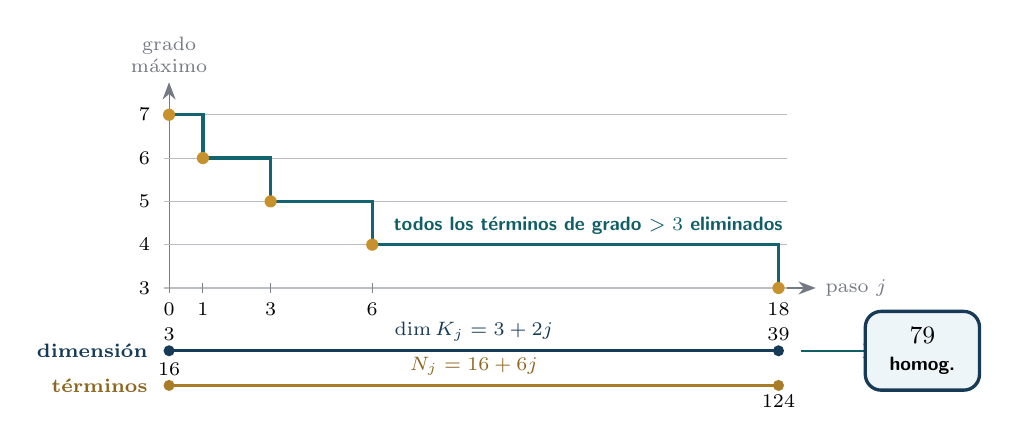
\begin{tikzpicture}[font=\small\sffamily]
  \begin{scope}[x=0.43cm,y=0.55cm]
    \draw[-{Stealth[length=2.2mm]},paperink!60] (0,0)--(19.1,0)
      node[right,font=\scriptsize] {paso $j$};
    \draw[-{Stealth[length=2.2mm]},paperink!60] (0,-0.1)--(0,4.75)
      node[above,font=\scriptsize,align=center] {grado\\m\'aximo};
    \foreach \d/\yy in {3/0,4/1,5/2,6/3,7/4}{
      \draw[paperink!30] (-0.15,\yy)--(18.25,\yy);
      \node[anchor=east,font=\scriptsize] at (-0.28,\yy) {$\d$};
    }
    \foreach \x in {0,1,3,6,18}{
      \draw[paperink!55] (\x,-0.12)--(\x,0.12);
      \node[below=2pt,font=\scriptsize] at (\x,0) {$\x$};
    }
    \draw[teal!80!black,very thick]
      (0,4)--(1,4)--(1,3)--(3,3)--(3,2)--(6,2)--(6,1)--(18,1)--(18,0);
    \foreach \x/\yy in {0/4,1/3,3/2,6/1,18/0}{
      \fill[gold] (\x,\yy) circle (2.2pt);
    }
    \node[anchor=west,font=\scriptsize\sffamily\bfseries,text=teal!75!black]
      at (6.35,1.45) {todos los t\'erminos de grado $>3$ eliminados};

    \draw[deepblue,very thick] (0,-1.45)--(18,-1.45);
    \fill[deepblue] (0,-1.45) circle (2pt);
    \fill[deepblue] (18,-1.45) circle (2pt);
    \node[anchor=east,font=\scriptsize\bfseries,text=deepblue]
      at (-0.35,-1.45) {dimensi\'on};
    \node[above,font=\scriptsize] at (0,-1.45) {$3$};
    \node[above,font=\scriptsize] at (18,-1.45) {$39$};
    \node[above,font=\scriptsize,text=deepblue] at (9,-1.45)
      {$\dim K_j=3+2j$};

    \draw[gold!85!black,very thick] (0,-2.25)--(18,-2.25);
    \fill[gold!85!black] (0,-2.25) circle (2pt);
    \fill[gold!85!black] (18,-2.25) circle (2pt);
    \node[anchor=east,font=\scriptsize\bfseries,text=gold!70!black]
      at (-0.35,-2.25) {t\'erminos};
    \node[above,font=\scriptsize] at (0,-2.25) {$16$};
    \node[below,font=\scriptsize] at (18,-2.25) {$124$};
    \node[above,font=\scriptsize,text=gold!70!black] at (9,-2.25)
      {$N_j=16+6j$};

    \draw[-{Stealth[length=2.4mm]},thick,teal!75!black]
      (18.65,-1.45)--(21.05,-1.45);
    \node[draw=deepblue,fill=softblue,rounded corners=2mm,very thick,
      minimum width=1.45cm,minimum height=10mm,font=\small\sffamily\bfseries,
      align=center] at (22.25,-1.45) {$79$\\[-0.1em]\scriptsize homog.};
  \end{scope}
\end{tikzpicture}
\caption{Perfil exacto de la reducci\'on de grado. Cada operaci\'on elemental
a\~nade dos variables y seis t\'erminos; los saltos efectivos de grado ocurren
en los pasos $1$, $3$, $6$ y $18$. La homogeneizaci\'on final lleva la
dimensi\'on de $39$ a $79$.}
\label{fig:bcw-profile}
\end{figure}

\begin{theorem}[Certificado c\'ubico homog\'eneo en dimensi\'on 79]
\label{thm:explicit-yagzhev}
El mapa
\begin{equation}\label{eq:explicit-yagzhev}
\mathcal Y(X,Y,T)=
\bigl(X+YT^2+A_2(X)T,\;Y-A_3(X),\;T\bigr)
\end{equation}
de $\C^{79}$ es identidad m\'as un vector homog\'eneo c\'ubico, satisface
$\det J\mathcal Y=1$ y no es inyectivo.
\end{theorem}

\begin{proof}
La parte no lineal es $(YT^2+A_2T,-A_3,0)$, homog\'enea de grado tres. La
construcci\'on de Bass--Connell--Wright aplicada a
\eqref{eq:K39-decomposition} prueba que su jacobiano es nilpotente y, por
tanto, $\det J\mathcal Y=1$.

Las tres colisiones racionales se transportan recursivamente: en el paso $j$,
$P\mapsto(P,-P_j(P),-Q_j(P))$. Sean $P_0,P_+,P_-\in\Q^{39}$ los puntos
obtenidos. Entonces
\[
K_{39}(P_0)=K_{39}(P_+)=K_{39}(P_-)
=\left(0,0,-\frac14,0,\ldots,0\right).
\]
Los tres puntos $(P_\varepsilon,A_3(P_\varepsilon),1)$ tienen la misma imagen
por $\mathcal Y$, luego $\mathcal Y$ no es inyectivo.
\end{proof}

El archivo \path{scripts/bcw_yagzhev_certificate.py} ejecuta las 18 operaciones
con aritm\'etica racional, verifica las colisiones y genera un certificado
autocontenido con las 79 coordenadas completas. De forma separada,
\path{scripts/verify_bcw_yagzhev_artifact.py} reconstruye la cadena desde el
JSON mediante una implementaci\'on propia de polinomios dispersos basada
\'unicamente en la biblioteca est\'andar de Python: no importa SymPy ni el
generador.

\begin{remark}[No minimalidad]
La dimensi\'on 79 certifica existencia expl\'icita, no optimalidad. Depende del
orden elegido para cancelar monomios y puede disminuir con factorizaciones
compartidas.
\end{remark}

\begin{figure}[htbp]
\centering
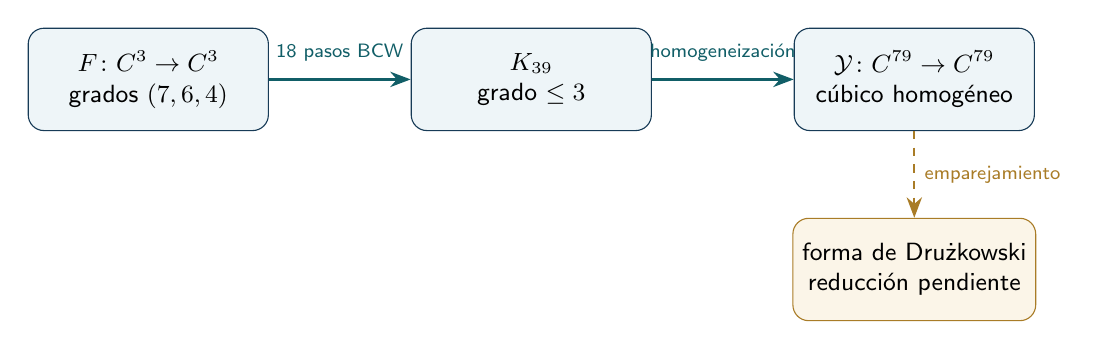
\begin{tikzpicture}[
  stage/.style={draw=deepblue,fill=softblue,rounded corners=2mm,
    minimum width=3.05cm,minimum height=13mm,align=center,font=\small\sffamily},
  openstage/.style={draw=gold!85!black,fill=softgold,rounded corners=2mm,
    minimum width=3.05cm,minimum height=13mm,align=center,font=\small\sffamily},
  arr/.style={-{Stealth[length=2.6mm]},thick,teal!75!black}
]
\node[stage] (f) {$F\colon\C^3\to\C^3$\\grados $(7,6,4)$};
\node[stage,right=18mm of f] (k) {$K_{39}$\\grado $\leq3$};
\node[stage,right=18mm of k] (y) {$\mathcal Y\colon\C^{79}\to\C^{79}$\\c\'ubico homog\'eneo};
\node[openstage,below=11mm of y] (d) {forma de Dru\.zkowski\\reducci\'on pendiente};
\draw[arr] (f)--node[above=1mm,font=\scriptsize\sffamily]{18 pasos BCW}(k);
\draw[arr] (k)--node[above=1mm,font=\scriptsize\sffamily]{homogeneizaci\'on}(y);
\draw[arr,dashed,gold!85!black] (y)--node[right,font=\scriptsize\sffamily]{emparejamiento}(d);
\end{tikzpicture}
\caption{Cadena constructiva de formas normales. Las dos primeras flechas se
ejecutan de forma exacta; la optimizaci\'on de Dru\.zkowski permanece abierta.}
\label{fig:bcw-reduction}
\end{figure}

\subsection{Qu\'e falta para una forma de Dru\.zkowski expl\'icita}

Dru\.zkowski demostr\'o que un mapa c\'ubico homog\'eneo puede emparejarse, en
dimensi\'on mayor, con uno c\'ubico-lineal \cite{Druzkowski1983,GorniZampieri1997}.
El Teorema~\ref{thm:explicit-yagzhev} entrega la entrada concreta, pero todav\'ia
falta descomponer los 124 monomios c\'ubicos en cubos de formas lineales,
construir las matrices de emparejamiento y eliminar variables redundantes.
No declaramos cerrada esa segunda reducci\'on.

\clearpage
\part{Consecuencias, verificaci\'on y perspectivas}

\section{Dixmier, Poisson y consecuencias l\'ogicas}

La Secci\'on~\ref{sec:what-changes} estableci\'o la cadena precisa
\[
\mathrm{JC}_{2n}\Longrightarrow
\mathrm{PC}_n\Longrightarrow
\mathrm{DC}_n\Longrightarrow
\mathrm{JC}_n.
\]
\begin{figure}[htbp]
\centering
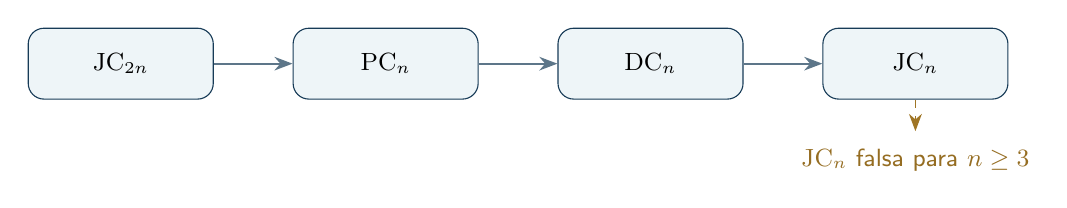
\begin{tikzpicture}[
  node distance=10mm,
  conjecture/.style={draw=deepblue,fill=softblue,rounded corners=2mm,
    minimum width=2.35cm,minimum height=9mm,font=\small\sffamily},
  arr/.style={-{Stealth[length=2.3mm]},thick,deepblue!70}
]
\node[conjecture] (jc2) {$\mathrm{JC}_{2n}$};
\node[conjecture,right=of jc2] (pc) {$\mathrm{PC}_n$};
\node[conjecture,right=of pc] (dc) {$\mathrm{DC}_n$};
\node[conjecture,right=of dc] (jc) {$\mathrm{JC}_n$};
\draw[arr] (jc2)--(pc);
\draw[arr] (pc)--(dc);
\draw[arr] (dc)--(jc);
\node[below=5mm of jc,text=gold!75!black,font=\small\sffamily]
  {$\mathrm{JC}_n$ falsa para $n\geq3$};
\draw[-{Stealth[length=2.2mm]},gold!80!black,dashed]
  (jc.south)--++(0,-4mm);
\end{tikzpicture}
\caption{Cadena l\'ogica que transporta la refutaci\'on hacia las conjeturas
de Poisson y Dixmier mediante contrapositiva.}
\label{fig:logical-consequences}
\end{figure}
Como $\mathrm{JC}_n$ es falsa para todo $n\geq3$, la contrapositiva muestra
que $\mathrm{DC}_n$ y $\mathrm{PC}_n$ son falsas para cada \`indice $n\geq3$.
En particular:

\begin{enumerate}
\item existen endomorfismos no invertibles del \`algebra de Weyl $A_n$ para
cada $n\geq3$;
\item existen endomorfismos no invertibles del \`algebra de Poisson can\'onica
de \`indice $n$ para cada $n\geq3$;
\item las versiones estables o ``para todo \`indice'' de ambas conjeturas son
falsas.
\end{enumerate}

Estas son consecuencias de existencia obtenidas mediante implicaciones entre
afirmaciones universales. No deben confundirse con la producci\'on inmediata de
endomorfismos peque\~nos y legibles. Traducir el presente mapa a testigos
expl\'icitos, controlar el aumento de grado y determinar el menor \`indice
posible son proyectos separados. Los casos de \`indice uno y dos no quedan
decididos por este contraejemplo.

\section{Componentes algebraicas y abundancia de contraejemplos}

Consideremos el espacio de mapas polin\'omicos de grado a lo sumo siete, que
fijan el origen y tienen determinante jacobiano uno. La versi\'on normalizada
$\widehat F$ pertenece a ese locus.

Un resultado reciente de Xavier afirma que, en cada componente irreducible de
un locus de mapas con $\det JF=1$, ocurre una dicotom\'ia: o todos los mapas de
la componente son automorfismos, o el miembro general no es un automorfismo
\cite{Xavier2026}.

\begin{corollary}[Consecuencia del principio de Xavier]
Toda componente irreducible del locus de Keller de grado a lo sumo siete que
contenga $\widehat F$ tiene miembro general no invertible.
\end{corollary}

Por tanto, el contraejemplo no deber\'ia concebirse como un punto aislado y
fr\'agil. Su mera presencia identifica componentes completas en las que la no
invertibilidad es el comportamiento gen\'erico. Una tarea prioritaria es
calcular la componente o las componentes que pasan por $\widehat F$, sus
dimensiones y deformaciones expl\'icitas.

\section{Formalizaci\'on, verificaci\'on y descubrimiento asistido}

El anuncio p\'ublico atribuy\'o el hallazgo del ejemplo a una consulta de Levent
Alp\"oge al sistema Fable \cite{AlpogeAnnouncement2026}. Paul Lezeau propuso
una versi\'on normalizada en Lean mediante una pull request que permanec\'ia
abierta y sin revisiones registradas en la fecha de este documento
\cite{LezeauLean2026}. Kevin Buzzard document\'o la verificaci\'on y su contexto inmediato
\cite{Buzzard2026}.

Conviene separar tres niveles:

\begin{enumerate}
\item \textbf{Descubrimiento:} encontrar los coeficientes y reconocer que el
mapa puede funcionar.
\item \textbf{Certificaci\'on:} comprobar el determinante y una colisi\'on
exacta; esta parte es corta y mecanizable.
\item \textbf{Comprensi\'on:} explicar la estructura, las fibras, el infinito,
las familias y las conexiones con otras conjeturas.
\end{enumerate}

La certificaci\'on formal reduce radicalmente el riesgo de un error algebraico,
pero no sustituye la etapa conceptual. El prop\'osito de este art\'iculo es
precisamente desarrollar esa comprensi\'on.

\section{S\'intesis de resultados}

\begin{center}
\begin{tabular}{@{}p{0.27\textwidth}p{0.64\textwidth}@{}}
\toprule
Estatus & Afirmaci\'on \\
\midrule
Demostrado & $\det JF=-2$ y existen tres preim\'agenes racionales de
$(-1/4,0,0)$. \\
Demostrado & La forma comprimida $F=(uq,y+3xq,xr)$ y la identidad
$x^2q=u+1-u^2r$. \\
Demostrado & La ecuaci\'on c\'ubica \eqref{eq:fibercubic} controla la coordenada
$x$ de toda fibra. \\
Demostrado & El grado gen\'erico es tres y el grupo de Galois gen\'erico es
$S_3$. \\
Demostrado & Tres es el menor grado gen\'erico posible de un contraejemplo;
todo contraejemplo de ese grado tiene cierre normal $S_3$. \\
Demostrado & La familia \eqref{eq:asymcurve} escapa al infinito con imagen
convergente en $\mathcal S$. \\
Demostrado & El conjunto exacto de no propiedad es
$\mathcal N_F=\mathcal S=\{D=0\}$. \\
Demostrado & $\Sing(\mathcal S)=\Gamma$ y
$F(\C^3)=\C^3\setminus\Gamma$. \\
Demostrado & El morfismo \eqref{eq:normalization-map} normaliza $\mathcal S$;
transversalmente a $\Gamma$ la singularidad es $X^2+Y^3=0$. \\
Demostrado & Las fibras tienen cardinalidad $3$, $1$ o $0$ sobre,
respectivamente, $\C^3\setminus\mathcal S$,
$\mathcal S\setminus\Gamma$ y $\Gamma$. \\
Demostrado & El mapa cu\'artico $F_4$ tiene determinante $-2$ y sus fibras
sobre $p\neq0$ est\'an controladas exactamente por las ra\'ices simples de
$\Omega_{p,q,r}$. \\
Demostrado & Para $F_4$, el conjunto omitido es estrictamente menor que el
locus singular del conjunto de no propiedad, al menos sobre $p\neq0$; en
particular, ambos conjuntos no son iguales. \\
Demostrado & Las 18 operaciones de la Secci\'on~\ref{sec:explicit-cubic}
producen un contraejemplo c\'ubico homog\'eneo expl\'icito en dimensi\'on 79. \\
Consecuencia formal & La conjetura es falsa en toda dimensi\'on $n\geq3$ y
en todo cuerpo de caracter\'istica cero. \\
Consecuencia formal & Bajo las convenciones de
\cite{AdjamagboVanDenEssen2007}, para cada \`indice $n\geq3$ las conjeturas de
Dixmier y Poisson correspondientes son falsas; tambi\'en fallan sus versiones
estables. \\
Consecuencia formal & La Vanishing Conjecture equivalente de Zhao es falsa en
alguna dimensi\'on. \\
Abierto & Determinar el grado m\'inimo de un contraejemplo en dimensi\'on tres. \\
Abierto & Resolver el caso de dimensi\'on dos. \\
Abierto & Extraer formas de Dru\.zkowski, Dixmier y Poisson expl\'icitas y
optimizar la forma c\'ubica homog\'enea de dimensi\'on 79. \\
\bottomrule
\end{tabular}
\end{center}

\section{Perspectivas y problemas abiertos}

Los resultados anteriores sustituyen varias preguntas iniciales por una
geometr\'ia concreta. Las direcciones siguientes recogen s\'olo los problemas
matem\'aticos que permanecen sustantivamente abiertos.

\subsection{Estratificaci\'on por multiplicidades en grado superior}

El Teorema~\ref{thm:quartic-separation} resuelve negativamente una pregunta
que surge de la geometr\'ia del ejemplo original: la igualdad entre conjunto
omitido y locus singular de no propiedad no es estable al pasar de grado
gen\'erico tres a cuatro. La siguiente etapa natural no consiste en repetir el
c\'alculo para ejemplos aislados, sino en formular para grado arbitrario una
estratificaci\'on por particiones de multiplicidades. En el abierto donde el
polinomio de fibras conserva su grado, la regla esperada es:
\begin{quote}
la cardinalidad de la fibra es el n\'umero de partes iguales a uno, mientras
que un valor es omitido exactamente cuando todas las multiplicidades son al
menos dos.
\end{quote}
El caso cu\'artico probado en la Secci\'on~\ref{sec:quartic} constituye el
primer test no trivial de este principio.

\subsection{Topolog\'ia de la frontera asint\'otica}

Aunque la imagen y el conjunto de no propiedad est\'an ahora determinados,
el Teorema~\ref{thm:normalization-cusp} cierra tambi\'en la normalizaci\'on, el
conductor y el tipo de singularidad transversal. Quedan los grupos
fundamentales, la monodrom\'ia topol\'ogica y el comportamiento de la cubierta
de tres hojas alrededor de la superficie.

\subsection{Clasificaci\'on de los contraejemplos de grado gen\'erico tres}

El Teorema~\ref{thm:generic-degree-three} fija grado m\'inimo tres, cierre
normal $S_3$ y ausencia de automorfismos de cubierta. El siguiente problema es
decidir cu\'anta rigidez geom\'etrica queda despu\'es de imponer esos datos.

\begin{question}
Sea $G\colon\C^n\to\C^n$ un mapa de Keller no automorfo de grado gen\'erico
tres. \`Es $G$, tras automorfismos polin\'omicos y estabilizaci\'on, equivalente
al mapa $F$ de este documento?
\end{question}

El grupo $S_3$ no determina el divisor en el infinito. Habr\'a que comparar la
normalizaci\'on y el conductor del conjunto de no propiedad, las componentes
omitidas, las valuaciones que pierden hojas y la monodrom\'ia local.

\subsection{El caso plano}

No se ha demostrado que un mapa de Keller plano no pueda tener grado
gen\'erico tres. Una obstrucci\'on v\'alida deber\'a usar geometr\'ia de ramas en
el infinito, dicriticales y topolog\'ia del conjunto de no propiedad.

\subsection{Compactificaci\'on}

Se debe extender $F$ a una aplicaci\'on racional entre compactificaciones
proyectivas, resolver sus indeterminaciones y describir los divisores del
infinito que dominan $\mathcal S$. La familia de la
Proposici\'on~\ref{prop:asymptotic} proporciona una carta inicial para esa
resoluci\'on.

\subsection{Monodrom\'ia y topolog\'ia}

Aunque el grupo gen\'erico $S_3$ ya est\'a identificado algebraicamente, queda
por describir la monodrom\'ia topol\'ogica mediante lazos expl\'icitos en el
complemento del discriminante. Esto deber\'ia explicar c\'omo se permutan las
tres ramas inversas.

\subsection{Deformaciones}

Hay que calcular el espacio tangente al locus $\det JF=1$ en $\widehat F$ y
buscar familias de coeficientes que preserven una colisi\'on o, m\'as
generalmente, grado gen\'erico mayor que uno. El principio de Xavier predice
abundancia gen\'erica en las componentes relevantes.

\subsection{Minimizaci\'on}

El ejemplo es lineal en $z$ y tiene grados $(7,6,4)$. Deben explorarse cambios
polin\'omicos y afines que reduzcan el n\'umero de monomios, la altura de los
coeficientes y el grado total. Tambi\'en es razonable buscar una clasificaci\'on
de mapas de Keller en tres variables lineales en una de ellas.

\subsection{Traducciones a otras conjeturas}

La primera traducci\'on hacia formas c\'ubicas est\'a implementada en el archivo
\begin{center}
\path{scripts/bcw_yagzhev_certificate.py}.
\end{center}
La cadena restante hacia
Dru\.zkowski, Dixmier, Poisson y Zhao debe implementarse con el mismo nivel de
verificabilidad.

\section{Limitaciones y alcance de las afirmaciones}

Este trabajo debe leerse con cuatro reservas expl\'icitas. Primero, el
contraejemplo, la nota p\'ublica y esta exposici\'on aparecieron en una ventana
temporal muy estrecha; por ello, toda afirmaci\'on de prioridad sobre los
resultados desarrollados aqu\'i es provisional y queda supeditada a una
b\'usqueda bibliogr\'afica m\'as amplia y a revisi\'on independiente
\cite{CounterexampleNote2026}.

Segundo, las identidades polin\'omicas centrales se verifican con aritm\'etica
exacta, pero el documento no constituye una formalizaci\'on integral en un
asistente de pruebas. La formalizaci\'on Lean citada es una propuesta externa
en una pull request abierta \cite{LezeauLean2026}.

Tercero, el mapa homog\'eneo de dimensi\'on $79$ es expl\'icito y
reproducible, pero no se afirma que esa dimensi\'on sea m\'inima. El certificado
comprueba las identidades de preservaci\'on del jacobiano, la estructura por
bloques y las colisiones racionales; su validez tambi\'en depende del teorema
general de homogeneizaci\'on de Bass--Connell--Wright.

Cuarto, el trabajo no resuelve el caso plano, no produce todav\'ia una forma
de Dru\.zkowski expl\'icita y no clasifica todos los mapas de Keller de grado
gen\'erico tres. Las preguntas de la secci\'on anterior deben entenderse como
programa de investigaci\'on, no como consecuencias ya establecidas.

\section{Conclusi\'on}

La conjetura jacobiana fall\'o exactamente en el salto de lo local a lo global.
El determinante constante controla toda la geometr\'ia infinitesimal, pero no
impide que varias hojas de una aplicaci\'on no propia se conecten a trav\'es del
infinito.

El mapa estudiado aqu\'i ofrece mucho m\'as que una refutaci\'on binaria. Posee
una estructura comprimida, una c\'ubica de fibras, monodrom\'ia gen\'erica
$S_3$, un conjunto exacto de no propiedad
$\mathcal S=\{D=0\}$ y una imagen exacta
$\C^3\setminus\Gamma$. Sus fibras se estratifican globalmente con
cardinalidades $3$, $1$ y $0$. Estas piezas constituyen ya una primera teor\'ia
concreta del contraejemplo, no s\'olo un certificado de su existencia.

La comparaci\'on cu\'artica aporta una primera correcci\'on a esa teor\'ia: la
curva omitida y el locus singular coinciden en el modelo c\'ubico porque un
polinomio c\'ubico singular sin ra\'ices simples debe tener una ra\'iz triple.
En grado cuatro aparece el tipo $3+1$: el discriminante es singular, pero la
ra\'iz simple restante conserva una preimagen. El infinito y la omisi\'on
quedan as\'i gobernados no s\'olo por la anulaci\'on del discriminante, sino por
la partici\'on completa de multiplicidades.

La normalizaci\'on identifica la frontera asint\'otica como una familia de
c\'uspides, mientras que la reducci\'on constructiva produce un testigo c\'ubico
homog\'eneo en dimensi\'on 79. En conjunto, estos resultados convierten un
certificado de no inyectividad en una primera teor\'ia concreta del mecanismo
global que hace posible el fallo.

Ahora sabemos que ``siempre'' era demasiado optimista. La nueva pregunta es
m\'as interesante: \emph{\`qu\'e condiciones adicionales distinguen las
aplicaciones de Keller globalmente invertibles de las cubiertas no propias de
varias hojas?}

\section*{Declaraciones acad\'emicas}
\addcontentsline{toc}{section}{Declaraciones acad\'emicas}

\textbf{Contribuci\'on del autor.}
Javier Arag\'on realiz\'o la organizaci\'on conceptual, los c\'alculos
adicionales, la implementaci\'on de los certificados, la redacci\'on y la
preparaci\'on editorial de esta exposici\'on independiente. La atribuci\'on del
descubrimiento del mapa se mantiene separada en la nota de procedencia.

\textbf{Uso de inteligencia artificial.}
Durante la investigaci\'on y preparaci\'on del manuscrito se utilizaron
asistentes de inteligencia artificial generativa para exploraci\'on
matem\'atica, programaci\'on simb\'olica, revisi\'on y edici\'on. Las
afirmaciones algebraicas presentadas como resultados se acompa\~nan de
demostraciones o certificados exactos reproducibles. La selecci\'on final de
las afirmaciones y la responsabilidad sobre el contenido corresponden al
autor.

\textbf{Disponibilidad de c\'odigo y artefactos.}
El paquete de esta versi\'on incluye
\path{scripts/bcw_yagzhev_certificate.py}, el verificador independiente
\path{scripts/verify_bcw_yagzhev_artifact.py}, la gu\'ia
\path{docs/REPRODUCIBILITY.md}, la especificaci\'on
\path{artifacts/bcw-yagzhev-certificate.schema.json}, el diccionario de campos
\path{artifacts/README.md}, el entorno documentado en
\path{environment.txt} y el certificado autocontenido legible por m\'aquina
\path{artifacts/bcw-yagzhev-dim79.json}. Este \'ultimo registra el mapa
original, su normalizaci\'on, los 18 pasos, la descomposici\'on intermedia, el
mapa final y dos representaciones de cada polinomio: una expresi\'on legible y
una lista can\'onica de coeficientes racionales con vectores de exponentes. El
archivo
\path{artifacts/SHA256SUMS} fija la integridad de los materiales distribuidos.
Los metadatos de citaci\'on se proporcionan en \path{CITATION.cff}. El DOI
reservado para esta versi\'on es \paperdoi; permanece pendiente de publicaci\'on
y no se presenta como enlace activo. La lista exacta de archivos y metadatos
del dep\'osito se fija en \path{docs/ARCHIVING.md}; la atribuci\'on detallada y
el alcance del certificado figuran en \path{docs/ATTRIBUTION.md} y
\path{docs/MATHEMATICAL_SCOPE.md}.

\textbf{Cita recomendada.}
J. Arag\'on, \emph{Ahora sabemos que ``siempre'' era demasiado optimista:
anatom\'ia algebraica y geom\'etrica de un contraejemplo expl\'icito a la
conjetura jacobiana}, versi\'on 1.0, 2026.
\par\noindent
DOI reservado, pendiente de publicaci\'on: \paperdoi.

\textbf{Financiaci\'on y conflictos de inter\'es.}
No se declara financiaci\'on externa espec\'ifica ni conflicto de inter\'es.

\textbf{Licencia.}
El texto y su fuente se distribuyen bajo CC BY 4.0; el c\'odigo y los
artefactos de verificaci\'on, bajo licencia MIT. Los t\'erminos completos se
incluyen en \path{LICENSE.md} y en el directorio \path{LICENSES/}.

\textbf{Agradecimientos.}
Se reconoce a Levent Alp\"oge por el anuncio p\'ublico, a Akhil Mathew por la
pregunta que lo motiv\'o, a Fable por el trabajo al que se atribuye el hallazgo
del ejemplo, a los autores de la nota p\'ublica contempor\'anea por su
exposici\'on algebraica, y a Paul Lezeau y Kevin Buzzard por la formalizaci\'on
propuesta y la documentaci\'on inmediata del resultado
\cite{AlpogeAnnouncement2026,CounterexampleNote2026,LezeauLean2026,Buzzard2026}.

\appendix

\section{Verificaci\'on simb\'olica reproducible}\label{app:reproducibility}

El siguiente guion de \texttt{SymPy} comprueba las identidades centrales. No
utiliza aritm\'etica de coma flotante.

\small
\begin{verbatim}
import sympy as s

x, y, z, a, b, c = s.symbols("x y z a b c")
u = 1 + x*y

F = s.Matrix([
    u**3*z + y**2*u*(4 + 3*x*y),
    y + 3*x*u**2*z + 3*x*y**2*(4 + 3*x*y),
    2*x - 3*x**2*y - x**3*z,
])

print(s.factor(F.jacobian([x, y, z]).det()))  # -2

A, B, C = F
D = 27*a**2*c**2 - 18*a*b*c + 16*a + b**3*c - b**2
E = 27*a*c**2 - 9*b*c + 8
P = D*x**3 + (4 - 3*b*c)*x - 2*c

print(s.factor(P.subs({a: A, b: B, c: C})))  # 0
print(s.factor(s.discriminant(P, x)))          # -4*D*E**2

G = s.groebner(
    [s.expand(A-a), s.expand(B-b), s.expand(C-c)],
    z, y, x,
    order="lex",
    domain=s.QQ.frac_field(a, b, c),
)
for polynomial in G.polys:
    print(s.factor(polynomial.as_expr()))
\end{verbatim}
\normalsize

Para verificar la familia asint\'otica se puede a\~nadir:

\small
\begin{verbatim}
lam, t = s.symbols("lam t", nonzero=True)
curve = {
    x: t,
    y: lam - 1/t,
    z: -3*lam/t + 5/t**2 - c/t**3,
}
print([s.factor(component.subs(curve)) for component in F])
\end{verbatim}
\normalsize

Las dos resultantes que cierran la imagen y el conjunto de no propiedad se
verifican mediante:

\small
\begin{verbatim}
U, lam = s.symbols("U lam")

R1 = U**2 - (1 + b*x)*U + 3*a*x**2
R2 = c*U**3 - x*U*(U + 1) + a*x**3
print(s.factor(s.resultant(R1, R2, U)))
# a*x**3*P

asym_a = a - lam**2*(1 - lam*c)
asym_b = b - lam*(4 - 3*lam*c)
print(s.factor(s.resultant(asym_a, asym_b, lam)))
# c*D
\end{verbatim}
\normalsize

La normalizaci\'on y la ecuaci\'on de la c\'uspide se comprueban mediante:

\small
\begin{verbatim}
h = 3*b*c - 4
print(s.factor(E**2 + h**3 - 27*c**2*D))  # 0

nu = {a: lam**2 - c*lam**3, b: 4*lam - 3*c*lam**2}
v = 3*c*lam - 2
print(s.factor(D.subs(nu)))                   # 0
print(s.factor(h.subs(nu) + v**2))            # 0
print(s.factor(E.subs(nu) + v**3))            # 0
print(s.factor((lam**2 - b*lam + 3*a).subs(nu)))  # 0
\end{verbatim}
\normalsize

Para reproducir todos los certificados de la Secci\'on~\ref{sec:quartic} se
puede ejecutar el siguiente bloque independiente:

\small
\begin{verbatim}
x, y, z, p, q, r, S, eps = s.symbols("x y z p q r S eps")

alpha = 1 + x*y
beta = alpha**2*z + y**2*(4 + 3*x*y)
P4 = alpha*beta
Q = y + 3*x*beta
R = 2*x - 3*x**2*y - x**3*z
F4 = s.Matrix([
    P4,
    Q + alpha**2*x**2*beta**4,
    R - s.Rational(1, 2)*x**4*beta**4,
])
print(s.factor(F4.jacobian([x, y, z]).det()))  # -2

Omega = (
    s.Rational(1, 2)*p**4*S**4 + 2*p*S**3
    - q*S**2 + 2*S - r
)
Delta4 = s.factor(s.discriminant(Omega, S))
H = s.factor(-Delta4/(4*p**2))
print(s.factor(Delta4 + 4*p**2*H))             # 0

squarefree_test = H
for variable in (p, q, r):
    squarefree_test = s.gcd(
        squarefree_test, s.diff(H, variable)
    )
print(s.factor(squarefree_test))               # 1

b = {p: 1, q: s.Rational(15, 4), r: s.Rational(11, 32)}
c = {p: 2, q: -s.Rational(17, 2), r: -2}
print(s.factor(Omega.subs(b)))
# (2*S - 1)**3*(2*S + 11)/32
print(s.factor(Omega.subs(c)))
# (4*S**2 + S + 2)**2/2
print(H.subs(b), [s.diff(H, v).subs(b) for v in (p, q, r)])
# 0 [0, 0, 0]

source_b = {
    x: s.Rational(11, 108), y: -10, z: -432864
}
print([s.factor(component.subs(source_b)) for component in F4])
# [1, 15/4, 11/32]

y_eps = 2*(1 - eps)
x_eps = 1/(2*eps)
z_eps = eps**3 - y_eps**2*(4 - y_eps/2)*eps
path = {x: x_eps, y: y_eps, z: z_eps}
print([s.factor(component.subs(path)) for component in F4])
# [1, 15/4 - 2*eps, 11/32 + eps/2]
\end{verbatim}
\normalsize

El certificado c\'ubico homog\'eneo se genera y verifica con:

\small
\begin{verbatim}
python scripts/bcw_yagzhev_certificate.py
python scripts/bcw_yagzhev_certificate.py --show-points
python scripts/bcw_yagzhev_certificate.py --show-components
python scripts/bcw_yagzhev_certificate.py \
  --write-artifact artifacts/bcw-yagzhev-dim79.json
python scripts/verify_bcw_yagzhev_artifact.py \
  artifacts/bcw-yagzhev-dim79.json
\end{verbatim}
\normalsize

La primera orden comprueba los determinantes $-2$ y $1$ del mapa original y de
su normalizaci\'on, las identidades de filas que preservan el determinante en
los 18 pasos, la dimensi\'on intermedia 39, los 124 t\'erminos, la identidad
jacobiana por bloques de la homogeneizaci\'on y las tres colisiones racionales
en dimensi\'on 79. Las dos \'ordenes siguientes imprimen los puntos y las
coordenadas completas; la cuarta genera el certificado JSON. La \'ultima lo
audita independientemente con aritm\'etica racional exacta, reconstruye los 18
pasos y el mapa final, y comprueba adem\'as los hashes de procedencia cuando
los archivos correspondientes est\'an disponibles.

\clearpage
\section*{Gu\'ia de lectura bibliogr\'afica}
\addcontentsline{toc}{section}{Gu\'ia de lectura bibliogr\'afica}

Las referencias se ordenan cronol\'ogicamente para mostrar la evoluci\'on del
problema. Las notas finales de cada entrada remiten a las p\'aginas de este
trabajo en las que se utiliza la fuente.

\begin{insightbox}{Mapa tem\'atico de las fuentes}
\renewcommand{\arraystretch}{1.28}
\begin{tabularx}{\textwidth}{@{}>{\raggedright\arraybackslash\sffamily\bfseries\color{deepblue}}p{0.29\textwidth}X@{}}
Fundamentos e historia &
Formulaci\'on, teorema de Ax--Grothendieck, genealog\'ia y referencia general:
\cite{Keller1939,Ax1968,VanDenEssen2000,RodriguezDiaz2026}.\\
\addlinespace[0.2em]
Criterios y geometr\'ia global &
Invertibilidad bajo hip\'otesis adicionales, caso galoisiano y no propiedad:
\cite{Campbell1973,Razar1979,Wang1980,Wright1981,Jelonek1993,Stacks0F2P}.\\
\addlinespace[0.2em]
Reducciones y formas normales &
Reducci\'on c\'ubica homog\'enea, forma de Dru\.zkowski y emparejamiento:
\cite{Yagzhev1980,BassConnellWright1982,Druzkowski1983,GorniZampieri1997}.\\
\addlinespace[0.2em]
Conjeturas equivalentes &
Dixmier, Poisson y formulaciones de anulaci\'on:
\cite{Zhao2004,BelovKanelKontsevich2007,AdjamagboVanDenEssen2007}.\\
\addlinespace[0.2em]
Contexto contempor\'aneo &
Principio organizador, nota matem\'atica, anuncio, propuesta Lean y contexto:
\cite{Xavier2026,CounterexampleNote2026,AlpogeAnnouncement2026,
LezeauLean2026,Buzzard2026}.\\
\end{tabularx}
\end{insightbox}

\begin{thebibliography}{99}

\bibitem{Keller1939}
\bibauthor{O.-H. Keller} (1939),
\emph{Ganze Cremona-Transformationen},
Monatshefte f\"ur Mathematik und Physik 47, 299--306.
\biblink{https://doi.org/10.1007/BF01695502}{DOI: 10.1007/BF01695502}

\bibitem{Ax1968}
\bibauthor{J. Ax} (1968),
\emph{The elementary theory of finite fields},
Annals of Mathematics 88, 239--271.
\biblink{https://doi.org/10.2307/1970573}{DOI: 10.2307/1970573}

\bibitem{Campbell1973}
\bibauthor{L. A. Campbell} (1973),
\emph{A condition for a polynomial map to be invertible},
Mathematische Annalen 205, 243--248.
\biblink{https://doi.org/10.1007/BF01349234}{DOI: 10.1007/BF01349234}

\bibitem{Razar1979}
\bibauthor{M. Razar} (1979),
\emph{Polynomial maps with constant Jacobian},
Israel Journal of Mathematics 32, 97--106.
\biblink{https://doi.org/10.1007/BF02764906}{DOI: 10.1007/BF02764906}

\bibitem{Wang1980}
\bibauthor{S. S.-S. Wang} (1980),
\emph{A Jacobian criterion for separability},
Journal of Algebra 65, 453--494.
\biblink{https://doi.org/10.1016/0021-8693(80)90233-1}{DOI: 10.1016/0021-8693(80)90233-1}

\bibitem{Yagzhev1980}
\bibauthor{A. V. Yagzhev} (1980),
\emph{Keller's problem},
Siberian Mathematical Journal 21, 747--754.
\biblink{https://doi.org/10.1007/BF00973892}{DOI: 10.1007/BF00973892}

\bibitem{Wright1981}
\bibauthor{D. Wright} (1981),
\emph{On the Jacobian conjecture},
Illinois Journal of Mathematics 25, 423--440.
\biblink{https://doi.org/10.1215/ijm/1256047158}{DOI: 10.1215/ijm/1256047158}

\bibitem{BassConnellWright1982}
\bibauthor{H. Bass, E. H. Connell y D. Wright} (1982),
\emph{The Jacobian conjecture: reduction of degree and formal expansion of
the inverse}, Bulletin of the American Mathematical Society 7, 287--330.
\biblink{https://doi.org/10.1090/S0273-0979-1982-15032-7}{DOI: 10.1090/S0273-0979-1982-15032-7}

\bibitem{Druzkowski1983}
\bibauthor{L. M. Dru\.zkowski} (1983),
\emph{An effective approach to Keller's Jacobian Conjecture},
Mathematische Annalen 264, 303--313.
\biblink{https://doi.org/10.1007/BF01459126}{DOI: 10.1007/BF01459126}

\bibitem{Jelonek1993}
\bibauthor{Z. Jelonek} (1993),
\emph{The set of points at which a polynomial map is not proper},
Annales Polonici Mathematici 58(3), 259--266.
\biblink{https://doi.org/10.4064/ap-58-3-259-266}{DOI: 10.4064/ap-58-3-259-266}

\bibitem{Pinchuk1994}
\bibauthor{S. Pinchuk} (1994),
\emph{A counterexample to the strong real Jacobian conjecture},
Mathematische Zeitschrift 217, 1--4.
\biblink{https://doi.org/10.1007/BF02571929}{DOI: 10.1007/BF02571929}

\bibitem{GorniZampieri1997}
\bibauthor{G. Gorni y G. Zampieri} (1997),
\emph{On cubic-linear polynomial mappings},
Indagationes Mathematicae 8, 471--492.
\biblink{https://doi.org/10.1016/S0019-3577(97)81552-2}{DOI: 10.1016/S0019-3577(97)81552-2}

\bibitem{VanDenEssen2000}
\bibauthor{A. van den Essen} (2000),
\emph{Polynomial Automorphisms and the Jacobian Conjecture},
Progress in Mathematics 190, Birkh\"auser.
\biblink{https://doi.org/10.1007/978-3-0348-8440-2}{DOI: 10.1007/978-3-0348-8440-2}

\bibitem{DeBondtVanDenEssen2005}
\bibauthor{M. de Bondt y A. van den Essen} (2005),
\emph{The Jacobian Conjecture for symmetric Dru\.zkowski mappings},
Annales Polonici Mathematici 86, 43--46.
\biblink{https://eudml.org/doc/280408}{EuDML: 280408}

\bibitem{DruzkowskiSymmetric2005}
\bibauthor{L. M. Dru\.zkowski} (2005),
\emph{The Jacobian Conjecture: symmetric reduction and solution in the
symmetric cubic linear case}, Annales Polonici Mathematici 87, 83--92.
\biblink{https://doi.org/10.4064/ap87-0-7}{DOI: 10.4064/ap87-0-7}

\bibitem{Zhao2004}
\bibauthor{W. Zhao} (2007),
\emph{Hessian nilpotent polynomials and the Jacobian Conjecture},
Transactions of the American Mathematical Society 359, 249--274;
prepublicaci\'on de 2004.
\biblink{https://arxiv.org/abs/math/0409534}{arXiv:math/0409534}

\bibitem{BelovKanelKontsevich2007}
\bibauthor{A. Belov-Kanel y M. Kontsevich} (2007),
\emph{The Jacobian Conjecture is stably equivalent to the Dixmier
Conjecture}, Moscow Mathematical Journal 7, 209--218.
\biblink{https://arxiv.org/abs/math/0512171}{arXiv:math/0512171}

\bibitem{AdjamagboVanDenEssen2007}
\bibauthor{P. K. Adjamagbo y A. van den Essen} (2007),
\emph{A proof of the equivalence of the Dixmier, Jacobian and Poisson
conjectures}, Acta Mathematica Vietnamica 32, 205--214.
\biblink{https://arxiv.org/abs/math/0608009}{arXiv:math/0608009}

\bibitem{Stacks0F2P}
\bibauthor{The Stacks Project Authors} (versi\'on consultada en 2026),
\emph{Applications of Zariski's Main Theorem, I}, Lemma 37.44.1, Tag 0F2P.
\biblink{https://stacks.math.columbia.edu/tag/0F2P}{Stacks Project: Tag 0F2P}

\bibitem{RodriguezDiaz2026}
\bibauthor{L. O. Rodr\'iguez D\'iaz} (2026),
\emph{On the origin of the Jacobian conjecture},
Comptes Rendus Math\'ematique 364, 363--370.
\biblink{https://doi.org/10.5802/crmath.831}{DOI: 10.5802/crmath.831}

\bibitem{Xavier2026}
\bibauthor{F. Xavier} (2026),
\emph{An organizing principle in the study of the Jacobian Conjecture},
arXiv:2606.22041, 20 de junio de 2026.
\biblink{https://arxiv.org/abs/2606.22041}{arXiv:2606.22041}

\bibitem{CounterexampleNote2026}
\bibauthor{Autor\'ia no indicada} (2026),
\emph{A Counterexample to the Jacobian Conjecture},
nota p\'ublica de siete p\'aginas, versi\'on consultada el 20 de julio de 2026.
\biblink{https://www.ulam.ai/research/jacobian.pdf}{Documento p\'ublico}

\bibitem{AlpogeAnnouncement2026}
\bibauthor{L. Alp\"oge} (2026),
\emph{Anuncio p\'ublico del contraejemplo atribuido a Fable},
20 de julio de 2026.
\biblink{https://x.com/__alpoge__/status/2079028340955197566}{Anuncio p\'ublico}

\bibitem{LezeauLean2026}
\bibauthor{P. Lezeau} (2026),
\emph{Propuesta Lean de una refutaci\'on de la conjetura jacobiana},
Google DeepMind Formal Conjectures, pull request 4474, abierta el 20 de julio
de 2026; estado consultado ese mismo d\'ia.
\biblink{https://github.com/google-deepmind/formal-conjectures/pull/4474}{Pull request 4474}

\bibitem{Buzzard2026}
\bibauthor{K. Buzzard} (2026),
\emph{Human mathematicians are being outcounterexampled},
Xena Project, 20 de julio de 2026.
\biblink{https://xenaproject.wordpress.com/2026/07/20/human-mathematicians-are-being-outcounterexampled/}{Nota de contexto}

\end{thebibliography}

\end{document}